\documentclass[12pt,
bibtotoc,liststotoc,appendixprefix
oneside,paper=a4,headings=small]{scrbook}
%
% Packages
% -----------------------------------
\usepackage[
  paper=a4paper,
  left=12.5mm,
  right=25mm,
  top=25mm,
  bottom=50mm,
  bindingoffset=10mm]{geometry}		% Seitenr�nder und Bindungskorrektur einstellen
  
\usepackage{apacite} 				% Literatur-Referenzen: American Psycholog. Assoc.
\usepackage{natbib}				
\usepackage{amsthm}	

%\setcitestyle{round,aysep={}} 		% Indizierg. in runden Klammern, zw. Autor u. Jahr
\setcitestyle{square}
%\usepackage[latin1]{inputenc} 		% Umlaute im Text
%\usepackage{ngerman}				% Rechtschreibg.
\usepackage[T1]{fontenc}
\usepackage{lmodern}				% Schriftfamilie
\usepackage{microtype}				% f�r die Mikrotypografie (besseres Schriftbild)
\usepackage[headsepline,footsepline]{scrpage2}

\usepackage{graphicx} 				% Grafiken einf�gen (pdf,png - aber jpg vermeiden)
\graphicspath{{./Bilder/}}          % Pfad zu den Bildern
\usepackage[export]{adjustbox}		% Positionieren von Bildern Tabellen
\usepackage{subfigure}				% L�sst Bilder nebeneinander darstellen
\usepackage{varwidth}
\usepackage{url}					% URL's formatieren (z.B. in Literatur) 
\usepackage[colorlinks,linkcolor=black,citecolor=black,urlcolor=black]{hyperref} 				% f�r Hyperlinks in PDF-Dokumenten
\usepackage{wrapfig}   
  
\usepackage{tabularx} 				% bessere Gestaltung von Tabellen
\usepackage{longtable} 		
\usepackage{multicol}				
\usepackage{multirow}
\usepackage{booktabs}
\usepackage{float}
\usepackage{framed}
\usepackage[labelfont=bf]{caption}
\usepackage{rotating}


\usepackage[table]{xcolor}

		
\usepackage[active]{srcltx}

\usepackage{listings}				% Algorithmen

\usepackage{mdwlist}				% Listen

\usepackage{setspace} 				% Zeileneinstellung
\newtheorem{mydef}{Merksatz}  		% Falls Beispiele, Merks�tze m. fortl. Nr. gebr. werden
\newtheorem{bsp}{Beispiel}

\usepackage{todonotes}				% zum Erstellen von ToDos im Editor

\usepackage{lscape}					% zum Rotieren von Seiten

\usepackage{amsmath}				% zum Schreiben von mathematischen Formeln

\usepackage{calc}

\usepackage{scrpage2}
\cfoot[]{}
\ofoot[\pagemark]{\pagemark}
\pagestyle{scrheadings}

%\usepackage{fancyhdr}

\usepackage{footnote}				% Fu�noten
\usepackage{tablefootnote}			% Fu�noten in Tabellen
\usepackage{amssymb}
%\clubpenalty = 10000
%\widowpenalty = 10000 \displaywidowpenalty = 10000

\hyphenation{voll-st\"andigen}		% Worttrennungen global definieren

\setcounter{tocdepth}{3}			% Ebenen, die im Inhaltsverzeichnis angezeigt werden

\theoremstyle{plain}
\newtheorem{thm}{Theorem}[chapter] % reset theorem numbering for each chapter

\theoremstyle{definition}
\newtheorem{defn}[thm]{Definition} % definition numbers are dependent on theorem numbers
\newtheorem{exmp}[thm]{Example} % same for example numbers

% Document
% -----------------------------------
\begin{document}
\parindent 0pt

\frontmatter 
    % Titelseite soll keine Kopf oder Fu�zeile haben
\thispagestyle{empty}

% Alle Elemente sollen zentriert sein


\begin{center}

\vspace*{-10mm}

%{\LARGE Freie Universit�t zu Berlin}\\

\vspace*{1cm}


\includegraphics[width=1.0\textwidth]{FULogo_Ausdruck_RGB}

\vspace*{1cm}

% Art der Arbeit => (Bachelorarbeit ,Diplomarbeit, Masterarbeit, Seminararbeit)
\Large \textbf{Masterthesis}\\ 

%\section*{\Large Masterthesis}

\vspace{1cm}

% Titel der Arbeit 
\LARGE \textbf{Inference of Boolean Networks considering real-life time 
course Data}\\ 

%\mdseries{Inference of Boolean Networks considering real-life time course Data}
%IBM Plex Serif Thin [OTF or TTF only] 

\vspace{1.5cm}

\Large Nina Valery Kersten\\


\parbox{120mm}{
\begin{large}
\begin{tabbing}
\textbf{Supervisors}\\\\
\hspace{.7cm} \= Prof. Dr. Heike Siebert\\
\hspace{.7cm} \= Prof. Dr. Alexander Bockmayr\\\\

\textbf{Advisor}\\\\
Phd. Robert Schwieger\\\\

\textbf{November 20, 2018} \\ 
\end{tabbing}
\end{large}
}

\end{center}
\clearpage{\pagestyle{empty}\cleardoublepage}
 			% Titelblatt
    \newpage
    \clearpage{\pagestyle{empty}\cleardoublepage}
    \thispagestyle{empty}


\vspace*{1cm}

\begin{center}
\textbf{Abstract}
\end{center}
%The survival of a cell and eventually of its organism depends mostly on  the reliable interaction between different kinds of substances. Different functionalities inside and outside a cell like profileration, division and apoptosis are part of different regulatory networks in a system. Small malfunction in these regulatory networks could cause diseases from low impact for the organism to a big one. Therefore it is necessary to learn these regulatory networks, its structure and dynamical behaviour for further drug design approaches. Several efforts have been made to infer a regulatory network.%Quellen. 
%In this work the focus is on inferring Boolean networks from real-life time-course data of breast cancer tissue, which provide a simplified version of the states of substances in a system (a gene is expressed:$1$, or not:$0$). The boolean network is validated for inferring the network by three inference different learning algorithms Reveal, Best-fit and Full-fit in combination with different k-means clustering binarization algorithms. The inferred networks are evaluated against a goldstandard to show how well the model predicted the networks structure. Thus, it is shown how the complexity and the size of a network influence the predictive power of the model and hence, the explanatory power of a boolean approach.

\vspace*{1cm}

\noindent 
%Give a short overview:
%Describe the Pipeline


    \newpage
    \clearpage{\pagestyle{empty}\cleardoublepage}
    \onehalfspacing                  	% Zeilenabstand ab hier 1.5 zeilig
    \tableofcontents 					% Inhaltsverzeichnis
    \clearpage{\pagestyle{empty}\cleardoublepage} 
    
    \listoffigures 					 	% Abbildungsverzeichnis
    \clearpage{\pagestyle{empty}\cleardoublepage}
    
    \listoftables						% Tabellenverzeichnis rein
    \clearpage{\pagestyle{empty}\cleardoublepage}
% -----------------------------------
\mainmatter 							% die einzelnen Kapitel
 	\chapter{Introduction and Review}

This chapter describes the different kinds of biological input data by taking a focus on the biological background of an experimental data set regarding protein-protein interaction of growth factor induced transcriptional signal pathways for inferring regulatory networks. The type of input data and its experimental data collection decides about the choice of an inference model and its interpretation.\\

Afterwards, biological data is put into a graph-theoretical context of a Boolean network. Additionally, this part shows how to capture the dynamics and structural properties of a Boolean network.

\section{Motivation}
%Biological motivation  
The development and functioning of a cell and its organism is a product of a complex cellular machinery, where the interaction of genes, proteins, \gls{mRNA} (messenger RiboNucleotide Acid) and metabolic substances take place in a cascade of extracellular signals transduced by mechanisms of the cell membrane, reaching the nucleus of the cell, initiating a transcription process that controls the production and abundance of proteins. Proper functioning of these regulatory networks is essential to the survival and adaptation of a cell. Malfunctioning has been identified as the cause of various diseases \citep{Berestovsky.2013}.
\\\\
Recent advances in high-throughput techniques provide a big abundance of information about various biological interaction measured over a series of time. It is necessary to handle this big data properly for significant structural and dynamic analysis. Therefore, experimental data is converted into a network structure, where a substance is represented by a node and an interaction is represented by an edge. Mostly substances are part of a big and highly interconnected system where the kinetic information is rarely known \citep{Saadatpour.2013}. Thus, the overall problem of inferring a regulatory network from biological time-course data is to find a trade-off between simplicity, scalability and explanatory power of a network, such that the main important components of a malfunctioning system can be identified for creating medical solutions \citep{Berestovsky.2013} \citep{Barman.2017}.
\\\\
%Different inference approaches of inference
Several models are known of inferring a network from time-course data, which are characterized being either continuous like Ordinary Differential Equation (ODE) models, Baysian models or discrete like Boolean networks (BN)\citep{Saadatpour.2013}. 
%Artificial Neural networks gather their knowledge by detecting patterns and relationships in data and learn through experience. An ANN is constructed by weighted processing elements which constitute the neural layers and are organized in layers. Thus the behaviour of a ANN is determined by a transition function of each variable (neuron), by a learning rule and by the architecture itself. A big advantage, no previous knowledge is needed %\citep{AGATONOVICKUSTRIN2000717}.\\

%Ordinary Differential Equations model
An Ordinary Differential Equation (ODE) creates networks considering kinetic properties of a biological system. This model is a powerful and flexible model to describe complex relations among substances. But kinetic information are rarly available, such that ODE is only a sufficient strategy when a small well known system is analyzed \citep{Saadatpour.2013}.
%\citep{}

%Baysian model
A Bayesian model is a graph-based model of joint multivariate probability distributions that captures properties of conditional independence between variables \citep{Friedman.2000}.\\\\

%Boolean model(BN)
Boolean network models are well known and do not need any kinetic information of a system. Hence, this model simplifies the representation of a complex system, while capturing the main structure and dynamics as well as the steady-state behaviour \citep{Berestovsky.2013}\citep{Saadatpour.2013}. Experimental settings are often financially expensive, such that the time course data sets are quite small. Boolean networks are known being able to derive relationships among substances from relatively small data sets (e.g. 50 measurements for one substance) \citep{Berestovsky.2013}. For this reason the Boolean network model is chosen in this thesis.
%What is a Boolean Network model?
In a Boolean network model, the initial state of a node is either true ($1$) or false ($0$) and the next state is updated according to a Boolean rule  composed by other nodes affecting the nodes state. Updating a nodes' state represents the measurement of sample points over a series of time, such that Boolean trajectories of the model are generated.
\\\\
In general, a pipeline for inferring Boolean networks starts with a normalized time-course data set, which is preprocessed by discretisizing continous values into binary values and remove redundant information. Subsequently,  an inference algorithm learns Boolean rules for each node from the data resulting in a set of rules. The predicted model is tested on itself and the predicted network is scored against a gold standard network.  
\\\\
This work is divided up into two parts for each a pipeline is implemented (available on Git: 'github.com/ninakersten/Masterthesis'). In the first part Boolean networks are learned from \textit{in silico} data sets of \textit{E.coli} and the mammilian cell cycle by three well known inference algorithms Best-Fit, Full-Fit and Reveal \citep{Barman.2017}. The predicted networks are scored against a gold standard, testing the inference algorithms and binarization algorithms on several parameters. 
%Gegen gold standard testen heißt: Predictive power zu ermitteln
%Wie kann die Güte beurteilt werden?Welche metriken gibt es?Wie vergleiche ich die netzwerke?
In the second part results about the algorithms' performance of the first part are taken into account for inferring a real-life time course data set of phophoprotein abundance measurements in breast cancer cell lines (Figure 1.1). This data is provided by the Reverse Engineering Assessment and Methods (DREAM)-Challenge platform. The DREAM-Challenge is a non-profit, collaborative community effort consisting of participants from across the research spectrum of questions in biology and medicine. On this platform real-life data is provided to everyone, such that everyone can participate by contributing own solutions and compare them to other researchers \citep{aboutdream, Bender.2016}.
    
\begin{figure}[H]
\captionsetup{width=0.9\linewidth}
\centering
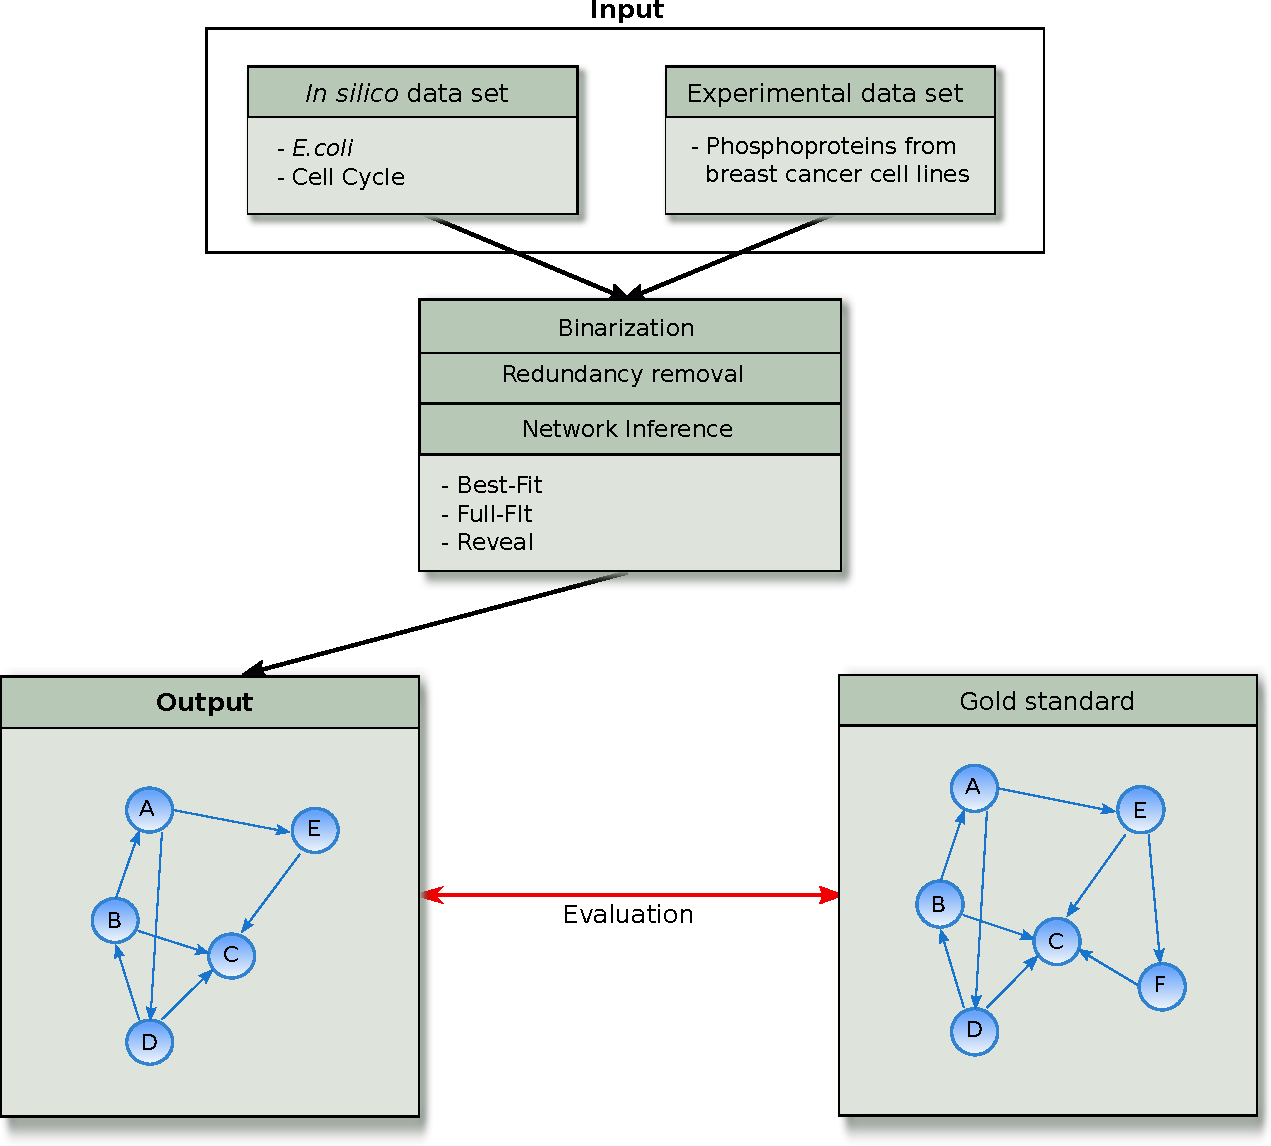
\includegraphics[width=0.8\textwidth]{./Bilder/motivation_pipeline.pdf}
\caption[Raw pipeline]{\textbf{Raw Pipeline.}Continuous input data of either E.coli, the cell cycle or of phosphoprotein interaction in breast cancer cell lines are binarized and redundant data is removed. A network is learned from an inference algorithm (e.g.: \textit{Best-Fit, Full-Fit, Reveal}), its predictive power is evaluated by scoring the output against a gold standard network. }
\label{fig:General Pipeline}
\end{figure} 

This thesis aims to show that a Boolean approach might be a sufficient strategy for inferring big real-life time course data sets by capturing the structure and dynamical properties of a system while emphasizing the limitations which might occur.


\newpage
\section{Biological Background}
%3 Levels of input data
Biological interaction can be observed at different levels of information integration of a cell regarding metabolic interaction, gene-gene interaction and protein-protein interaction.\\ 
%Signal integration
Information integration starts with a signal, which binds to a membrane integrated receptor of the cell causing an activation of one or multiple target proteins inducing several signal transduction cascades (Figure 2.1). While the signal is transduced, it is amplified by enzymatic activities or inhibited by feedback pathways down the cascade. Finally transcription factors are activated by the input signal, such that the expression of a target gene by generating mRNA results in a protein. The resulting proteins influence the cell's survival by its proliferation, induction of cell differentiation and apoptosis.


\begin{figure}[H]
%\setlength{\abovecaptionskip}{0pt}
\captionsetup{width=1.0\linewidth}
\centering
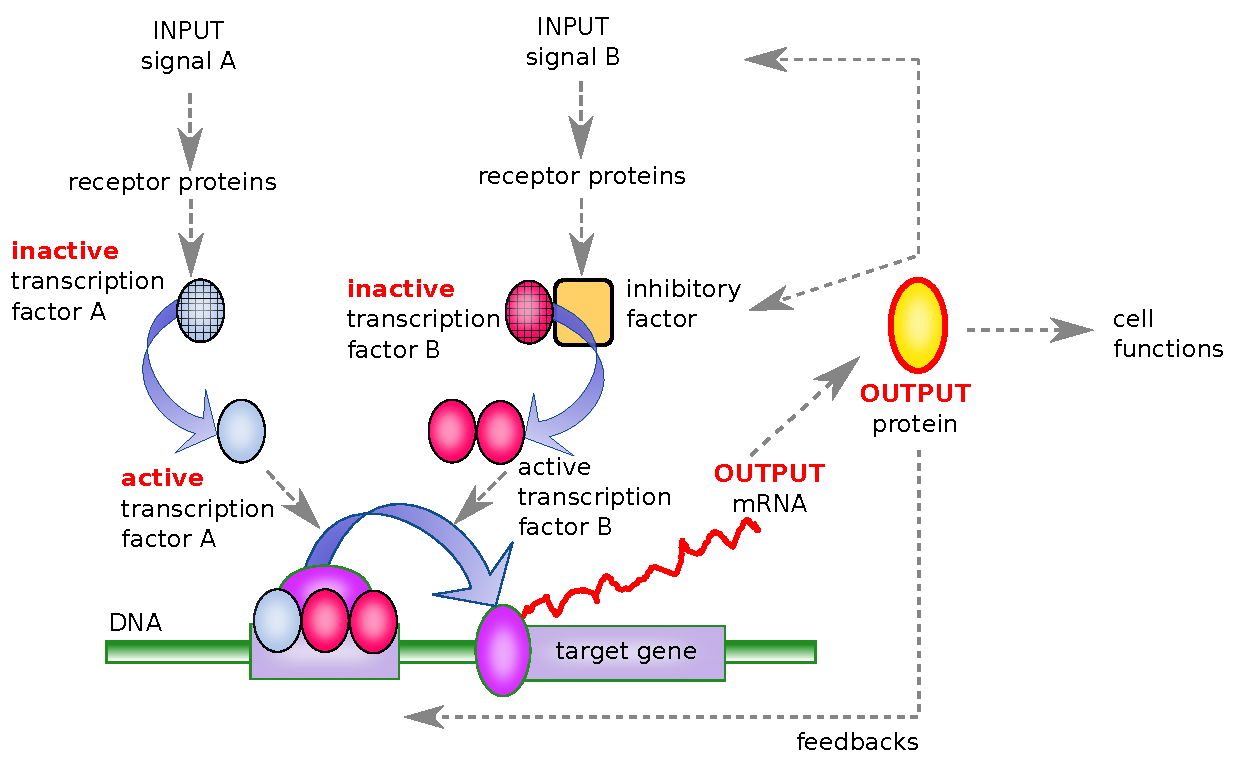
\includegraphics[width=0.85\textwidth]{./Bilder/GRN.pdf}
%\setlength{\abovecaptionskip}{-5ex}
\caption[Transcriptional Signal Cascade]{\textbf{Transcriptional Signal Cascade}
Two different input signals $A$ and $B$ bind to a specific receptor protein. The complex of $A$ activates the transcription factor $A$ that binds directly to the gene's regulatory sequence inducing the expression of the target gene. Different to $A$ initiates the complex of $B$ a separation of the inactive $B$ (\textit{pink oval}) from an inhibitory factor (\textit{yellow rectangle}). Transcription factor $B$ is then free to bind to the cis-regulatory sequence. Thus the expression level of this target gene is leveled by signal $A$ and $B$. The mRNA output results in a protein product which can take place in several processes of the cell \citep{U.S.DepartmentofEnergyOfficeofScience.April2001}.}
%\setlength{\belowcaptionskip}{0pt} 
\label{fig:Fig.2.}
\end{figure}


The concentration of substances in signalling pathways underlies high fluctuation over time due to transcriptional and translational regulation, such that the inference of a significant network is a challenging task \citep{Kestler.2008, Oates.2012}.

\subsection*{Metabolic network}

At the level of metabolic networks the substances are highly interconnected in a quite complex way (e.g. cell respiration in Figure 1.3). An individual's metabolism is determined by its genetics, environment and nutrition.\citep{Shmulevich.2002}. In a metabolic network the nodes are depicted by different types of biochemical components connected by directed edges describing a activating or inactivating interaction. Biochemical reaction are represented by a metabolic pathway, which consists of a sequence of biochemical reactions that produce a set of metabolites from a set of precursor metabolites and cofactors. The length of a pathway is the number of biochemical reactions between the precursor and the final metabolites of the pathway \citep{Shmulevich.2003}. 
%The definition of a pathway is not unique, therefore the length of pathways vary. 

\begin{SCfigure}[][!h]
%\centering
%\captionsetup{width=.7\linewidth}
\begin{minipage}{0.65\linewidth}
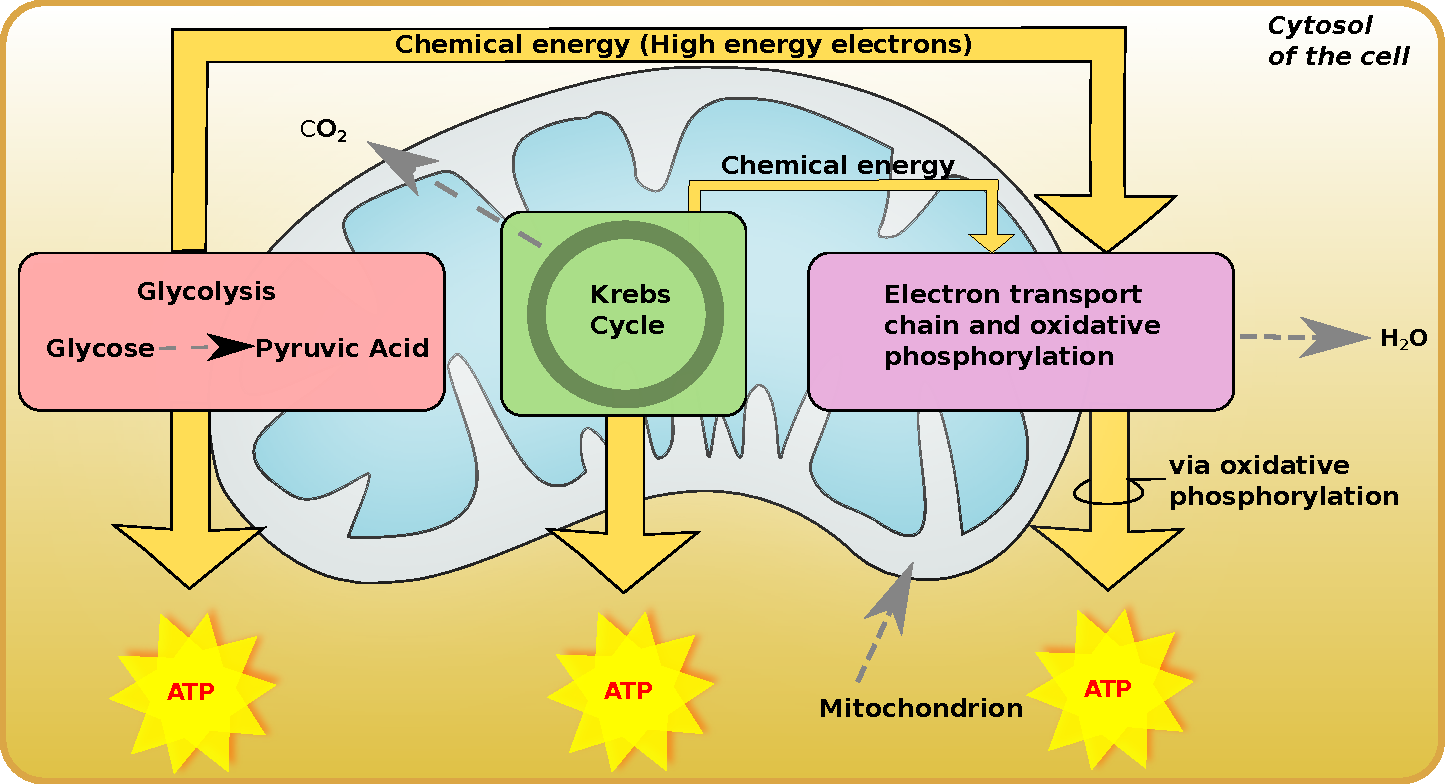
\includegraphics[width=1.0\textwidth]{./Bilder/metabolic.pdf}
\end{minipage}
%\begin{minipage}{width=0.3\textwidth}
\caption[Metabolic Network for cell respiration]{\textbf{Metabolic Network for cell respiration. } In a mitochondrion, an essentiell compartment of the cell, converts energy derived from nutrition into biochemical energy \gls{ATP}(Adenosin TriPhosphate) by releasing waste products of water $H_{2}O$ and $CO_{2}$.}
%\end{minipage}
\label{fig:Fig.3.}
\end{SCfigure} 
\citep{cellrespiration}


\subsection*{Gene regulatory network}

In a gene regulatory network (\gls{GRN}) depicted in Figure 1.2 the interaction of genes are identified indirectly by the abundance measurement of their transcriptional products (e.g. mRNA, proteins). The nodes of a GRN are depicted by the genes' names and the edges are directed by showing whether a gene produces proteins which inhibit or activate a target gene  \citep{Karlebach.2008}.



%\newpage
\subsection*{Protein-Protein-Interaction network}
In contrast to the gene regulatory interaction network in a protein-protein interaction (\gls{PPI}) network the proteins act directly among themselve. Thus the nodes in a network are the interacting proteins. Proteins interact by physical contacts (e.g. electrostatic forces) of high specificity. PPIs play a big role in electron transfer, signal transduction, transport across the membrane and cell metabolism. The underlying assumption is that true interactions are likely to occur between proteins involved in the same biological process, proteins found in the same cell compartment, and proteins whose mRNA are co-expressed \citep{LasRivas.2010}\citep{Pellegrini.2004}.\\

The real-life data set of the DREAM-Challenge used in this work is dealing with PPIs, thus, it is important to know for later data collection, data processing and discussion how the data is obtained and which role these PPIs play in a biological context.\\

Referring to the general description of a transcriptional signal cascade (Figure 1.2) we state the receptor being an enzyme-associated receptor and the input signals are growth factors. An enzyme associated receptor has a polypeptide chain integrated in the cell's membrane with a tyrosine kinase activity (Figure 1.4).


\begin{figure}[H]
%\setlength{\abovecaptionskip}{0pt}
\captionsetup{width=.9\linewidth}
\centering
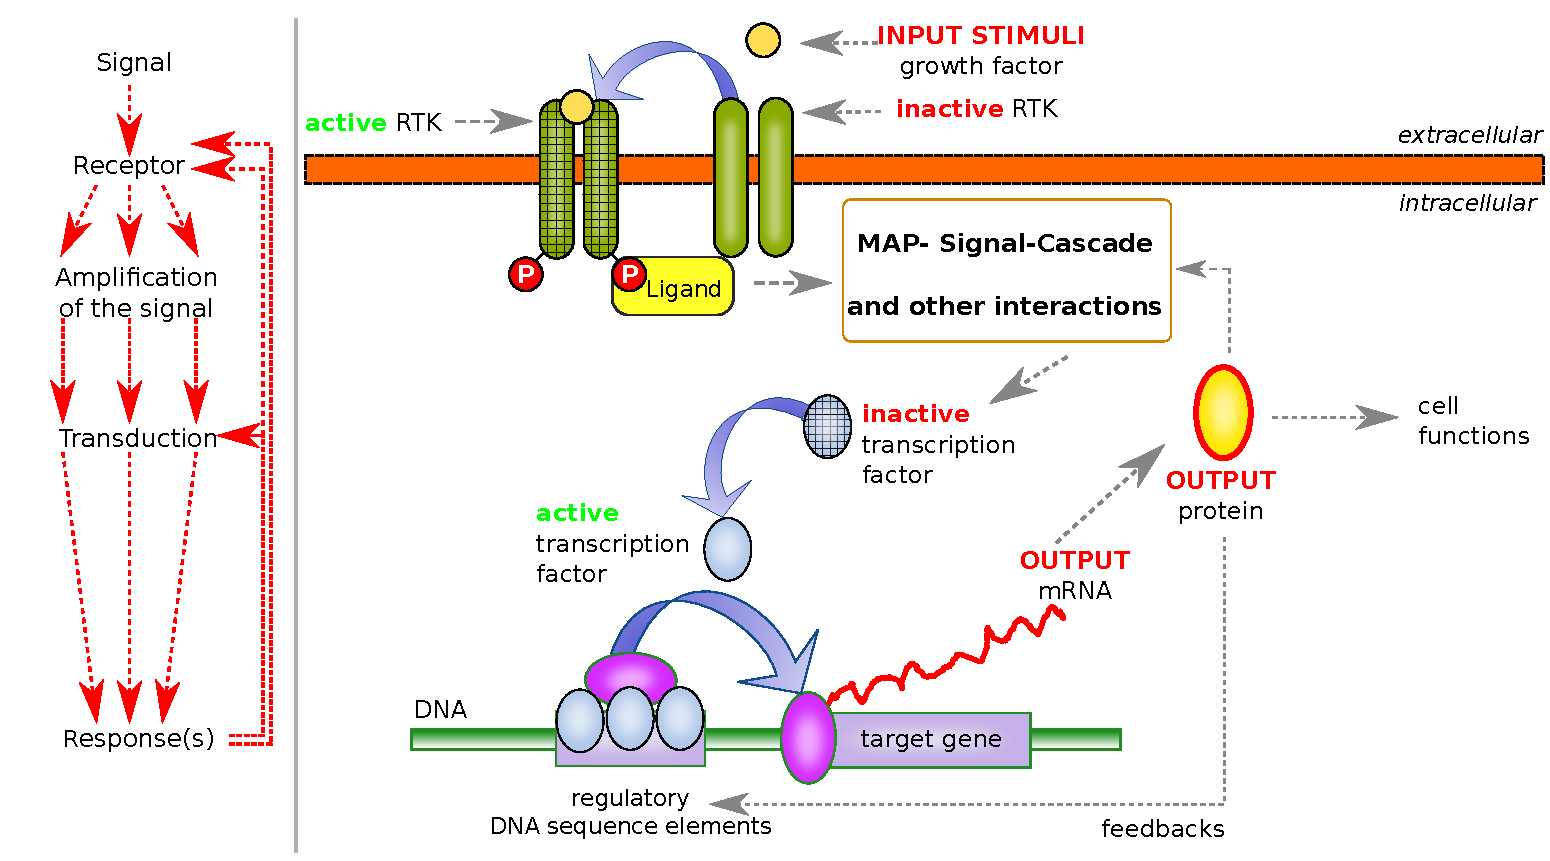
\includegraphics[width=0.8\textwidth]{./Bilder/GRNDREAM8.pdf}
%\setlength{\abovecaptionskip}{-5ex}
\caption[Transcriptional Signale Cascade of RTKs]{\textbf{Transcriptional Signale Cascade} An incoming stimuli (\textit{yellow circle}) representing a growth factor binds to an inactive RTK (\textit{green}), such that the RTK is activated. The RTK amplifies the signal and initiates a signal transduction cascade, such that an inactive transcription factor (\textit{blue oval}) is activated, which binds to regulatory DNA sequence elements inducing the mRNA transcription of a target gene resulting in a new protein \citep{U.S.DepartmentofEnergyOfficeofScience.April2001}. }
%\setlength{\belowcaptionskip}{0pt} 
\label{fig:DREAM8GRN}
\end{figure}


Growth factor receptors with a tyrosine kinase activity are called receptor tyrosine kinases (\gls{RTK}s). These RTKs have the property of autophosphorylation, meaning that they amplify their incoming signal. Binds a ligand to this receptor, first the receptor autophosphorylates and then phosphorylates the tyrosin residues of the ligand. By the phosphorylation of the receptor and several other ligands (resp. proteins) a phosphorylating cascade (e.g. signal transduction cascade) is induced. In this mitogen activated protein (MAP) phosphorylation cascade the \gls{MAP}-kinase katalyzes the phosphorylation of effector proteins, such that inactive transcription factors are activated starting the transcription process of a target gene and finally resulting in a protein product \citep{MullerEsterl.2009}.\\

\newpage
In the DREAM-Challenge growth factors are selected depicted as a stimuli by pertubating the cell's signal transduction. Thus, different stimuli cause different signal transduction cascades. Depending on the incoming stimuli particular proteins take place in the signal transduction cascade. The goal is to figure out PPIs in this phosphorylation cascade by inferring a Boolean network based on the measurement of the proteins abundance considering eight different incoming growth factors (resp. stimuli) displayed in Table 1.1. 
dysregulation of the genes of these growth factors have been linked to diseases such as cancer, schizophrenia, bipolar disorder and many more \citep{NRG1}.


%{\tabcolsep=2.5pt%
\begin{center}
\captionsetup{width=0.87\linewidth}
%\setlength\extrarowheight{4pt}
%\noindent\begin{tabular}{c|c|l}
%\def\arraystretch{2.0}%
\scriptsize
%\addtolength{\tabcolsep}{-5pt}
\begin{tabular}{lll}
\toprule 
 Notation & Name & Description\\
\hline\hline
IGF1 & Insulin like Growth Factor 1 & \parbox{8cm}{Hormone, similar to the insulin function and structure \citep{IGF1}}\\
\midrule NRG1 & Neuregulin 1 & \parbox{8cm}{Membrane glycoprotein, mediating cell-cell signalling, critical role in growth and developement of the cell \citep{NRG1}}\\
\midrule HGF & Hepatocyte Growth Factor & \parbox{8cm}{Regulate cell growth, cell motility and morphogenesis \citep{HGF}} \\
\midrule FGF1 & Fibroblast Growth Factor 1 & \parbox{8cm}{Functions as a modifier of endothelial cell migration, proliferation and an angiogenic factor\citep{FGF1}}\\
\midrule Insulin & Insulin & \parbox{8cm}{Mutations in this gene are associated with type II diabetes and susceptibility to insulin resistance \citep{Insulin}}\\
\midrule EGF & Epidermal Growth Factor & \parbox{8cm}{This protein acts a potent mitogenic factor that plays an important role in the growth, proliferation and differentiation of numerous cell types \citep{EGF}.}\\
\midrule PBS & Translocator Protein (TSPO) &  \parbox{8cm}{Present mainly in the mitochondrial compartment of peripheral tissues. The protein is a key factor in the flow of cholesterol into mitochondria to permit the initiation of steroid hormone synthesis \citep{PBS} \citep{PBS}.}\\
\midrule Serum & SRF & \parbox{8cm}{Member of the MADS box superfamily
of transcription factors \citep{Serum}}\\
\bottomrule
\end{tabular}
\captionof{table}{List of growth factors (stimuli) of DREAM8 Challenge}
%List of growth factors (resp. hormons) used in the Dream8 Challenge. All of them take place in the regulation of the cell's functions. Malfunctioning of these signals may cause several diseases (e.g. cancer).}
\end{center}
%}


%\newpage
%RPMA vllt. besser in den Teil: Data collection of DREAM8-Challenge packen?
\subsubsection*{Reverse phase Protein lysate MicroArray}
One of the most effetive strategy to collect data of protein-protein interaction is a technique so called reverse phase protein lysate microarray(\gls{RPMA}, resp. RPPA). RPMA is an antibody-based assay that provides quanitative measurements of protein abundance \citep{authornamenotavailable.}.
This technique is divided up into 6 parts. First starting with the sample collection. An inhibitor or stimulus in form of drugs is added to a set of cell lines at the same time and the cell lines are then processed at different time points. Secondly in the cell lyses step cell fragments are lysed with a cell lysis buffer to obtain high protein concentration. The choice of a buffer decides the quantity of proteins that can be lysed out of the cell. Afterwards cell lysed probes are diluted. In the Antibody screening the lysates are pooled and resolved by \gls{SDS-PAGE} (Sodium Dodecyl Sulfate - Polyacrylamide Gel Electrophoresis) followed by western blotting on a nitrocellulose membrane \citep{AlTubuly.2000}. The membrane is cut into 4mmm strips. Each slide is probed with a different antibody, where a primary antibody is extended by a secondary antibody. For fluorometric detection primary and secondary antibody are diluted (Figure 1.5). %A detection reagent is put on each slide. Signal amplification and detection is done by an optical flatbed scanner if colormetric technique is used or by laser scanning. 
The resulting data is normalized, such that outliers are excluded from the data's structure \citep{Boellner.2015}.\\

\begin{SCfigure}[][!h]
	%\setlength{\abovecaptionskip}{0pt}
	%\captionsetup{width=0.7\linewidth}
	%\centering
	\begin{minipage}{0.6\linewidth}
	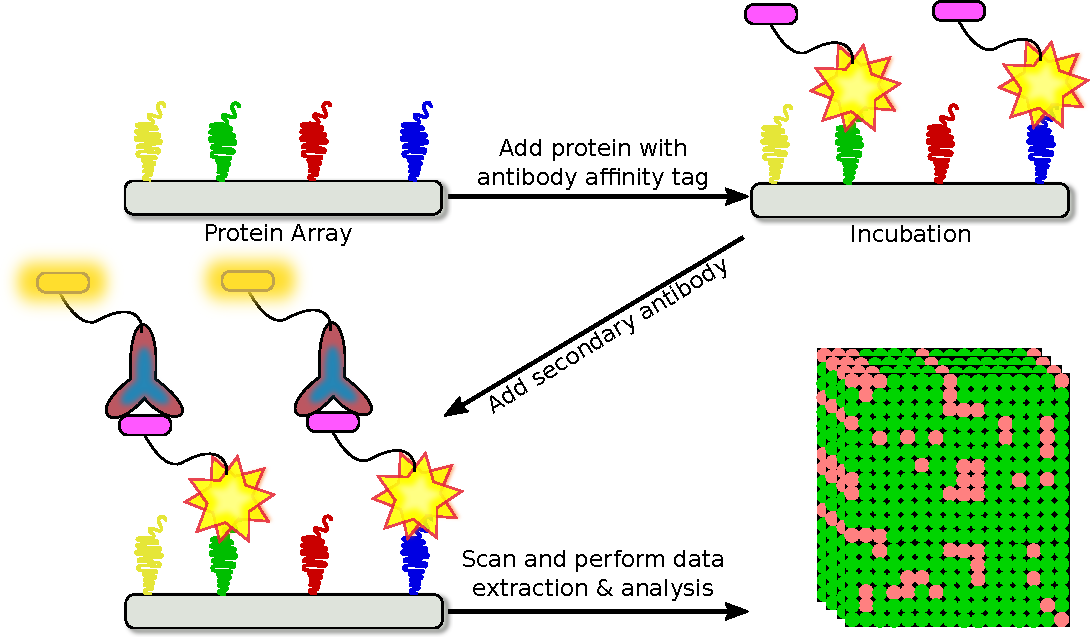
\includegraphics[width=0.9\textwidth]{./Bilder/RPMA.pdf}
	\end{minipage}
	%\setlength{\abovecaptionskip}{-5ex}
	\caption[RPMA: Antibody binding and fluorometric detection]{\textbf{RPMA: Antibody binding and fluorometric detection.} Proteins are tagged by a specific antibody. After incubation time the secondary antibody is added. Finally the abundance of proteins is determined by a fluorometric detection.}
	%\setlength{\belowcaptionskip}{0pt} 
	\label{fig:Fig.4}
\end{SCfigure}

The strength of RPMA is the high throughput, ulta-sensitive detection of proteins from extremely small numbers of input material which is not possible for western blotting and \gls{ELISA} (Enzymatic Immunoassay) \citep{Boellner.2015}. The small spot size on the microarray, ranging in diameter from 85 to 200 micrometres, enables the analysis of thousands of samples with the same antibody in one experiment \citep{Ramaswamy.2005}. The high sensitivity of RPMA allows for the detection of low abundance proteins or biomarkers such as phosphorylated signaling proteins from very small amounts of starting material such as biopsy samples, which are often contaminated with normal tissue\citep{Sheehan.2005}. A great improvement of RPMAs over traditional forward phase protein arrays is a reduction in the number of antibodies needed to detect a protein \citep{Sheehan.2005, Liotta.2003}. The protein isn't detected directly which helps to preserve the proteins. Antibodies, especially phospho-specific reagents, often detect linear peptide sequences that may be masked due to the three-dimensional conformation of the protein. This problem is overcome with RPMA as the samples can be denatured, revealing any covered epitopes (part of a protein recognized by specific antibody)\citep{Liotta.2003}.\\

The weakness of RPMA are batch effects caused by the choice of the right buffer, quantity of the proteins and the antibody performance.
The choice of the right buffer decides the quantity of proteins which can be lysed out of the cell. Little or poor quality of starting material and a long storage time causes low protein. It might be useful to improve the antibody performance by validating it with a smaller sample size under identical conditions before starting with the actual sample collection. Currently the number of signalling proteins for which antibodies exist to get an analyzable signal is quite small. \\

\newpage
\section{Graph-theoretical Background}
This section is dealing with defining the graph-theoretical properties of a Boolean network $N$ in terms of its structure and dynamics.\\


\begin{defn}
\textbf{Boolean Network}\\
\textit{A Boolean network $N$ is defined by an n-dimensional binary vector $X=(x_{1},...,x_{n})$, where each element $x_{i}\in X$ corresponds to the state $x_{i}=1$ or $x_{i}=0$ of a species $i$. Then a set $F$ of $n$ transition functions contains a particular function $f_{i}$ for each species $x_{i}$ \citep{Berestovsky.2013}. 
Every transition function $f_{i} \in F$ is therefore a n-variable Boolean function $f:\mathbb{B}^{n} \rightarrow \mathbb{B} $, which is represented by a Boolean expression over $n$ input variables \citep{HannesKlarner.November2014}.
\\For every $f_{i}\in F$ s.t. $1\le i\le n$,
\begin{equation}
f_{i}(X(t))=x_{i}(t+1)
\end{equation}
, where $f_{i}(X(t))$ defines the next state for each $x_{i}$ at time $(t+1)$ in the network.}
\end{defn}


In a biological context the activity of a node is a qualitative rate whether a gene is being transcribed $x_{i}=1$ or not $x_{i}=0$, a transcription factor is active or inactive, a protein's concentration is above or below a certain threshold (e.g. phosporylated or un-phosphorylated). Thus a network with $n$ nodes will have $2^{n}$ possible states.
\citep{Saadatpour.2013}\citep{Lahdesmaki.2003}\citep{HannesKlarner.November2014T}.
\\
Then a transition $f_i$ describes a rule of $n$ node defining by their activating or inhibitory influence on a target node the next state of a that node \citep{Berestovsky.2013}.\\

For instance, a gene $x_{A}$ is activated by another gene $x_{B}$ and inhibited by a second gene $x_{C}$. Then the transition function of $x_A$ is $f_{x_{A}}=x_{B} \land  \neg x_{C}$ and the Boolean algebra looks like this;

\hspace{-15px}
\begin{equation}
\begin{split}
x_{A}& = x_{B} \text{ \&\&  !} x_{C} 
\end{split}
\end{equation}

, where a Boolean function is a composition of nodes $x_{i}\in X$ and logical operators represented by '\&\&', '||', '!' (resp. 'NOT', 'AND' and 'OR' ;resp. '$\land$' ,'$\lor$' , '$\neg$') \citep{Saadatpour.2013}\citep{Berestovsky.2013}. \\

A Boolean network can be abstracted into a graphical representation of an interaction graph capturing the structural properties of it. Therefore the notation of a directed graph is introduced.

\newpage
\begin{defn}
\textbf{Directed Graph}\\
\textit{A directed graph $G=(V,A)$ is an ordered pair, defined as a set of nodes $V=\{v_{1},v_{2},...,v_{n}\}$ and a set of directed edges $A$ denoted as 'arcs'. A set of directed edges $A=\{ (i,j)|i,j\in V\} $ describes the flow of information in a network, where $(i,j)$ describes a flow from $i$ (tail) to $j$ (head)} (Figure 1.6).\\
\end{defn} 
\citep{Pavlopoulos.2011}

\begin{defn}\textbf{Interaction Graph}\\
\textit{The interaction graph (\gls{IG}) (resp. dependency raph) of a Boolean network $N$ is a directed graph $IG(X,A)$ that consists of the node set $X$ and the arc set $A = A _{F} \subseteq X \times X$ with $(x_{i},x_{j})\in A \text{ iff }f_{x_{j}}$ depends on $x_{i}$, then:}
\end{defn} 
\begin{equation}
a_{ij}=\begin{cases}
1 & \text{ if there is an edge from node i to node j}\\
0 & \text{ otherwise}
\end{cases}
\end{equation}
\citep{HannesKlarner.November2014T}
%(Gutes Paper mit Definitionen:!!!!!\citep{Pavlopoulos.2011})

\begin{SCfigure}[][!h]
	%\begin{figure}[H]
	\begin{minipage}{0.4\linewidth}
	%\vspace{-\baselineskip}
	%\captionsetup{width=0.7\linewidth}
	\hspace{30px}
	%\centering
	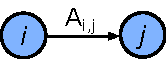
\includegraphics[width=0.5\textwidth]{./Bilder/DirectedGraph.pdf}
	\end{minipage}
	\caption[Directed Graph \textit{G}]{\textbf{Directed Graph \textit{G}. }$a_{i,j}$ is a directed edge (arc) depicting the flow of information from node $i$ to node $j$.}
	\label{fig:7}
\end{SCfigure}
%\end{figure}

In an interaction graph for each node being described by another one, this connection is written '$x_{i}$ $1$ $x_{j}$' and for the case that there is no connection '$x_{i}$ $0$ $x_{j}$', respectively.
\\\\
Furthermore an interaction graph provides information about nodes having a positive or negative influence on other nodes depicted by the \textit{Sign} of an edge. This term is introduced for completion and is not necessary for later investigation in this thesis. 

\begin{defn}\textbf{\textit{Sign} of an edge}\\
\textit{The sign of an edge is defined by $Sign(x_{i}\rightarrow x_{j}) \subseteq \{+,-\}$.}
\end{defn}

Then the expression $x_{i}\rightarrow x_{j}$ is either $x_{i}\xrightarrow{+}  x_{j}$ (resp. $x_{i}$ $1$ $x_{j}$) describing an activating connection, $x_{i}\xrightarrow{-} x_{j}$ (resp. $x_{i}$ $-1$ $x_{j}$ ) describing an inhibitory connection or both $x_{i}\xrightarrow{+,-} x_{j}$ (resp. $x_{i}$ $1,-1$ $x_{j}$ ).\\

\begin{SCfigure}[][!h]
\begin{minipage}{0.4\linewidth}
%\captionsetup{width=0.9\linewidth}
%\vspace{-10px}
%\centering
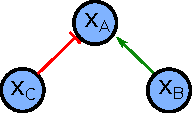
\includegraphics[width=0.58\textwidth]{./Bilder/Interactiongraph1.pdf}
\end{minipage}
\caption[Interaction graph \textit{G}]{\textbf{Interaction graph \textit{IG}. }Relating to the Boolean rule (1.2) a node $x_{A}$ is activated (\textit{green}) by $x_{B}$ and inhibited (\textit{red}) by $x_{C}$.}
\label{fig:7}
\end{SCfigure}

 
The number of incoming edges of a node denoted by the \textit{\textbf{in-degree}} of a node is a sufficient parameter for complexity analysis in a network. 

\begin{defn}\textbf{\textit{In-degree}}\\
The \textit{in-degree} of a node is the number of incoming edges to a node determining its state.
\begin{equation}
k^{in}_{i}=\sum_{j}{a_{ij}}
\end{equation}
\end{defn}
\citep{Barman.2017, NykampDQ.hiddene}
%(Gutes Paper mit Definitionen:!!!!!\citep{Pavlopoulos.2011})
Hence, the out-degree describes the number of outgoing edges of a node. Nodes with only outgoing edges (in-degree$=0$) are called sources, and nodes with only incoming edges (out-degree$=0$) are sinks of the network. The higher the \textit{in-degree} of a node, the more nodes are part of its transition function $f$ and the complexity increases. Here, the \textit{in-degree} of $x_{A}$ in Figure 1.7 is $k^{in}_{x_{A}}=2$.\\

%It is desireable to determine the nodes whos \textit{in-degree} is the highest among other nodes, whose removal can break down the network into isolated clusters \citep{Albert.2002}. 
%\begin{defn}\textbf{Indegree}\\
%\textit{}
%\end{defn}

Furthermore the dynamics of a system (resp. the state change behaviour of a node over a series of time) can be simulated by repeatedly applying the set $F$ of transition functions to the corresponding set of nodes $X$ and updating their 'current' state \citep{Berestovsky.2013}.\\
In a \textit{\textbf{synchronous}} simulation, the states of all nodes are updated simultaniously after all transition function of $F$ have been applied to all nodes $X$. In contrast to the \textit{\textbf{asynchronous}} simulation, the states are updated by randomly choosing a transition function $f_{i}\in F$ and updating the state of $x_{i}$ in the exact time \citep{Hopfensitz.2012, Liang.1998, Lahdesmaki.2003, Albert.2008}.
In biological processes interaction of substances rarely happen at the same time, thus dynamical analysis is an important factor of detecting interacting substances.
\\\\
These two terms of updating a node's state are abstracted in a so called \textit{state transition graph} \citep{Saadatpour.2013}.

\begin{defn}\textbf{State Transition Graph}\\
\textit{A state transition graph (\gls{STG}) is a directed graph with a set of nodes represented by a set of binary vectors $F(t+1)=\{ f_{1}(X(t+1)),...,f_{n}(X(t+1))\}$, representing the updated states of all variables after all of the functions in $F$ have executed. The arcs denote possible transitions from one binary state vector to another}.
\end{defn}
\citep{Saadatpour.2013, Lee.2002, HannesKlarner.}
%\raggedbottom
\\
Starting from an initial state in the state transition graph and iteratively updating the state of the nodes, the state of the system evolves over time by following a trajectory of states until the nodes' states do not change anymore: $X(t)=X(t+1)$ , so called \textbf{\textit{steady-state}} \citep{Saadatpour.2013, Liang.1998}. These steady-states describe the 'true' state of the nodes in a system, thus the 'true' connection of the nodes to each other. 
\\\\
The following example demonstrates deriving $F$ from an interaction graph $IG$, calculating the corresponding set of binary trajectories $B=\{B_{1},...,B_{n}\}$ (one per species) updated in a synchronous and asynchronous manner resulting in two state transition graphs.
\\\\
\textbf{Example 1.1} The interaction graph in Figure 1.8 shows a Boolean network with three nodes $X=\{x_{1},x_{2},x_{3}\}$ (\textit{blue circle}), where positive (resp. activating) edges (\textit{green}) and negative (resp. inhibiting) edges (\textit{red}) represent the interaction between the nodes. The \textit{in-degree} of $k^{in}_{x_{1}}=2$, $k^{in}_{x_{2}}=1$ and $k^{in}_{x_{3}}=3$.

 
\begin{figure}[H]
\centering
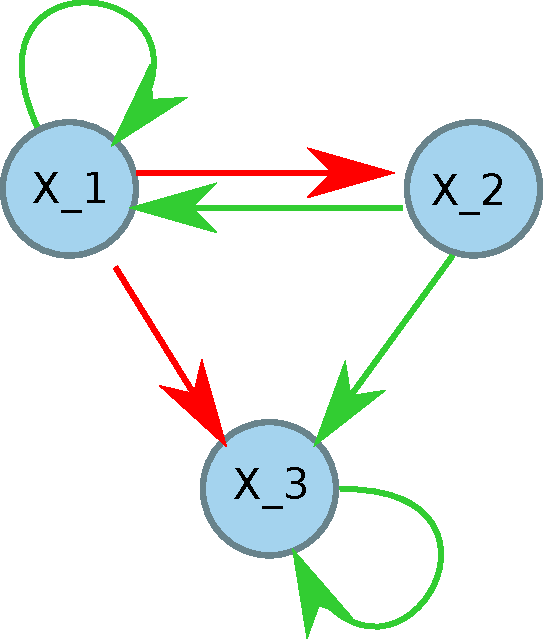
\includegraphics[scale=1.2]{./Bilder/examplenetwork.pdf}
%\end{minipage}
\caption[Interaction Graph]{\textbf{Interaction Graph}}
\label{fig:IG}
\end{figure}
%Graphik und caption an die Breite der seite anpassen


From the interaction graph the set of transition functions $F$ (resp. Boolean functions) can be derived (1.6) such that the state transition graph can be calculated.

\begin{equation}
F(x_{1,2,3}) = 
\begin{pmatrix}
x_1      & \land & x_2 & \land &\neg x_3\\
\neg x_1 &       &      &       & \\
         &       & x_2  &\land & x_3
\end{pmatrix}
\end{equation}


For every possible state of $x_i\in X$ the next state $f_{i}(X(t))=x_{i}(t+1)$ is calculated shown in the computation (1.7)-(1.14) below \citep{Remy.2008}.


\begin{align}
x(t)& =(0,0,0) &\rightarrow & &f(x(t+1)) = (0,1,0)\\
\color{red}x(t)& \color{red}=(0,0,1) &\color{red}\rightarrow & &\color{red}f(x(t+1)) = (0,1,0)\\
x(t)& =(0,1,0) &\rightarrow & &f(x(t+1)) = (0,1,0)\\
x(t)& =(1,0,0) &\rightarrow & &f(x(t+1)) = (0,0,0)\\
x(t)& =(1,1,0) &\rightarrow & &f(x(t+1)) = (1,0,0)\\
\color{red}x(t)& \color{red}=(1,0,1) &\color{red}\rightarrow & &\color{red}f(x(t+1)) = (0,0,0)\\
x(t)& =(0,1,1) &\rightarrow & &f(x(t+1)) = (0,1,1)\\
\color{red}x(t)& \color{red}=(1,1,1) &\color{red}\rightarrow & &\color{red}f(x(t+1)) = (0,0,1)
\end{align}

As we know from the description of asynchronous STG's in biological systems processes happen uncommonly at the same time, which is observed by comparing state transition graph of the synchronous (A) and asynchronous (B) model in Figure 1.9. In contrast to the synchronous STG where each state has a unique successor, in the asynchronous STG multiple successors of a trajectory are possible (e.g. (1.8),(1.12),(1.14)) \citep{Saadatpour.2013}. 

\begin{figure}[H]
  \centering
% \begin{varwidth}{\linewidth}
    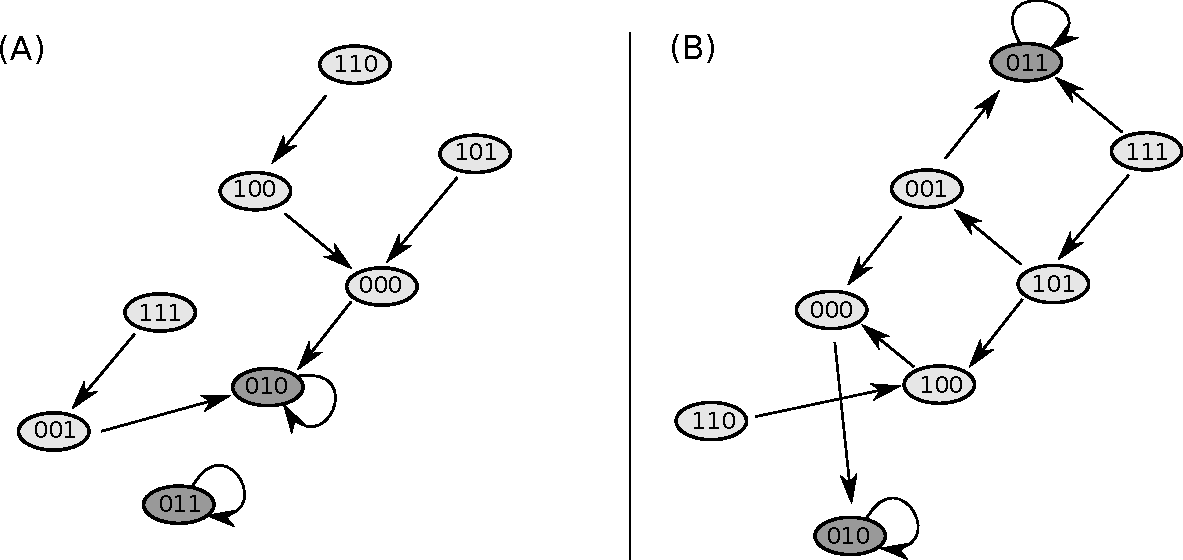
\includegraphics[scale=.7]{./Bilder/asynchronexample.pdf}
  %\end{varwidth} % ein Leerzeichen Abstand
  %\begin{varwidth}{\linewidth}
   % 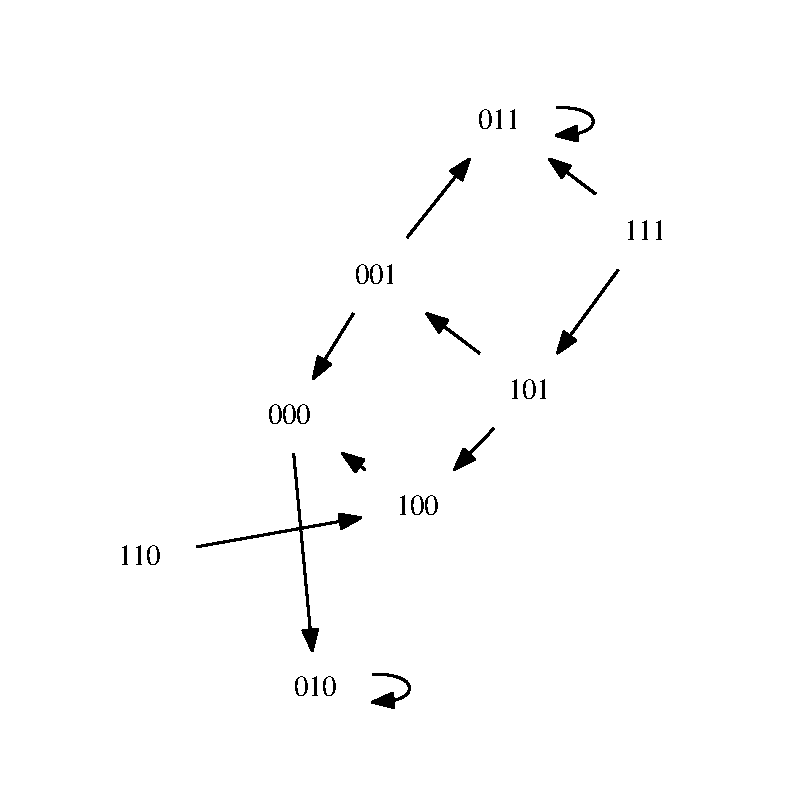
\includegraphics[scale=.6]{./Bilder/example01_asynchron_stg}
 % \end{varwidth}
  \caption[Synchronous and Asynchronous State Transition Graph]{\textbf{Synchronous and Asynchronous State Transition Graph}. (A): Synchronous state transition graph; and (B): Asynchronous state transition graph of a Boolean network. Binary digits from left to right depict the state of the nodes $x_1$,$x_2$,$x_3$. The dark gray states are possible steady-states in the system.}
\label{fig:Fig.4.}
\end{figure}


%S (set of states),B(binarized boolean trajectories),k(indegree value),n(number of nodes),m(number of measurements) Begriffe einführen
%\\newpage



    \clearpage{\pagestyle{empty}\cleardoublepage}
    \chapter{Background}



\section{Biological Background}

Depending on the aim of a network inference the biological input data can be depicted by the interaction of proteins, genes and metabolic substances. In this section the intention of using different types of input data is explained and what potentially will be the occuring problems. Different types of biological input data provide different structures of the input data for further network inference algorithms. 

\newpage

\subsection*{Transcriptional Gene Regulatory Networks}

In a Transcriptional Gene regulatory network (GRN) the nodes are depicted by the genes and the arcs are directed and show whether a gene produces RNA (transcript of the source gene,resp. regulator) which inhibits oder activtes the target gene (regulatee). For network inference computational algorithms take the mRNA expression levels of genes as the input data. %\citep{https://www.nature.com/articles/nrm2503}.
 
\begin{figure}[H]
%\setlength{\abovecaptionskip}{0pt}
\centering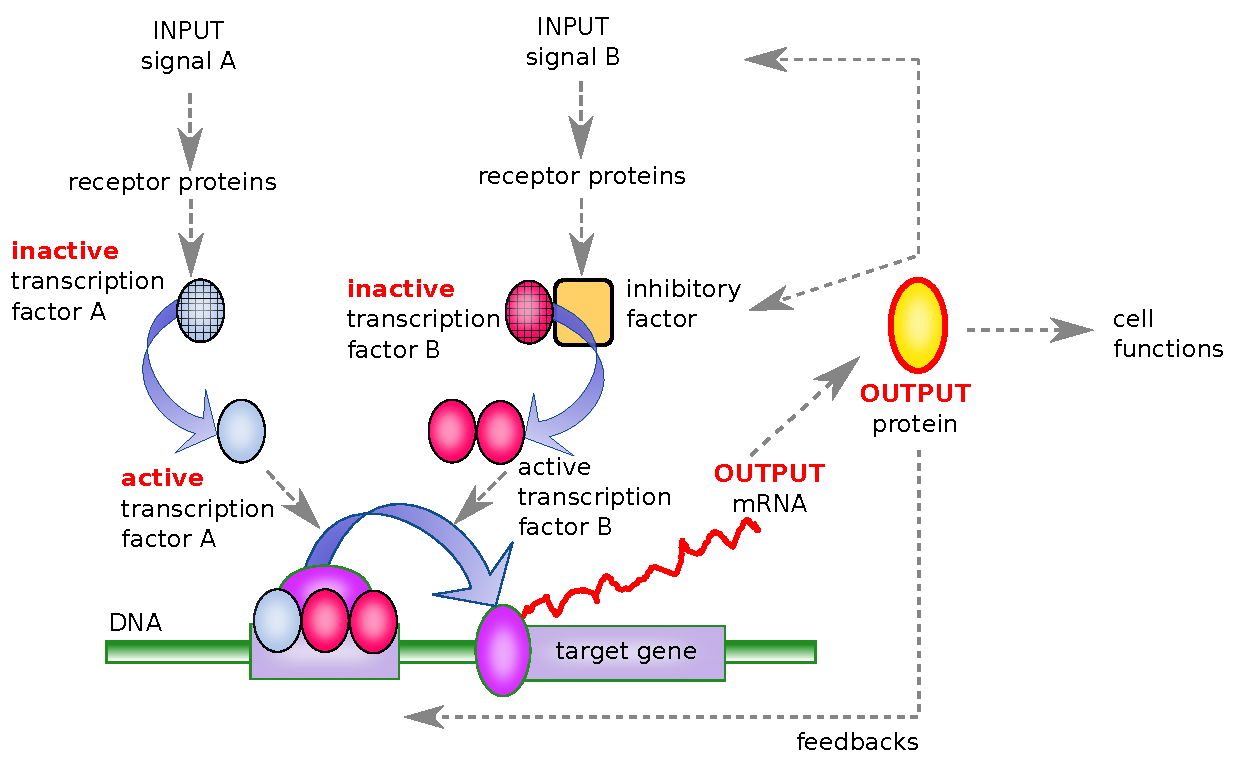
\includegraphics[width=1.3\textwidth]{./Bilder/GRN}
\caption[Transcriptional Gene Regulatory Network (GRN)]{\textbf{Transcriptional Gene Regulatory Network (GRN).}

In this example two different signals have an impact of a single target gene. Signal molecule A triggers the conversion of inactive transcription factor A (green oval) into an active form that binds directly to the target gene's cis-regulatory sequence. The process for signal B is more complex. Signal B triggers the separation of inactive B (red oval) from an inhibitory factor (yellow rectangle). B is then free to form an active complex that binds to the active A transcription factor on the cis-regulatory sequence. The net output is expression of the target gene, leveled by A nd B. Thus cis-regulatory DNA sequences with the proteins that assemble on them, integrate information from multiple signaling inputs to produce mRNA-Output . 
\citep{https://public.ornl.gov/site/gallery/detail.cfm?id=302&topic=&citation=&general=gene20regulatory20network&restsection=all} }
%\setlength{\belowcaptionskip}{0pt} 
\label{fig:Fig.2.}
\end{figure}


\subsection*{Metabolic Interaction}
Metabolic interactions represent the most complex cellular processes. Connections between biochemical reaction via substrate and product metabolites create complex metabolic networks.
The focus is set on the different aspects of enzyme chemistry, enzymestructure and metabolite structure. Thus an individual's metabolism is determined by one's genetics, environment, and nutrition. By investigating the chemical structure of metabolites and systematically classify the functions of the enzymes the understanding of a metabolism and the prediction of enzyme function and novel metabolic pathways is improved.\citep{104(6):1777-1782}\citep{HATZIMANIKATIS2004300}

\newpage

\subsection*{Signal Transduction}

In the developement of multicellular organisms the action of extracellular growth factors activate a cascade of intracellular signaling pathways. These pathways regulate major aspects of cell regulation like cell profileration, cell migration, cell differentiation,cell survival and cell death. To understand the developement of diseases (e.g. cancer) major prozesses (e.g. phosphorylation, ubiquitylation, methylation, etc.) of signal transduction pathways can be delightet by the prediction of a network . In signal transduction proteins are the nodes and directed edges represent interaction, where the biochemical modification of the regulatee is changed by the impact of the regulator. The concentration of signalling pathway underlies high fluctuation over time due to transcriptional and translational regulation, such that the inference of a network is a challenging task \citep{BIES:BIES20834}
%\citep{https://www.ncbi.nlm.nih.gov/pmc/articles/PMC3436851/}.


\begin{figure}[H]
\centering
%\setlength{\abovecaptionskip}{0pt}
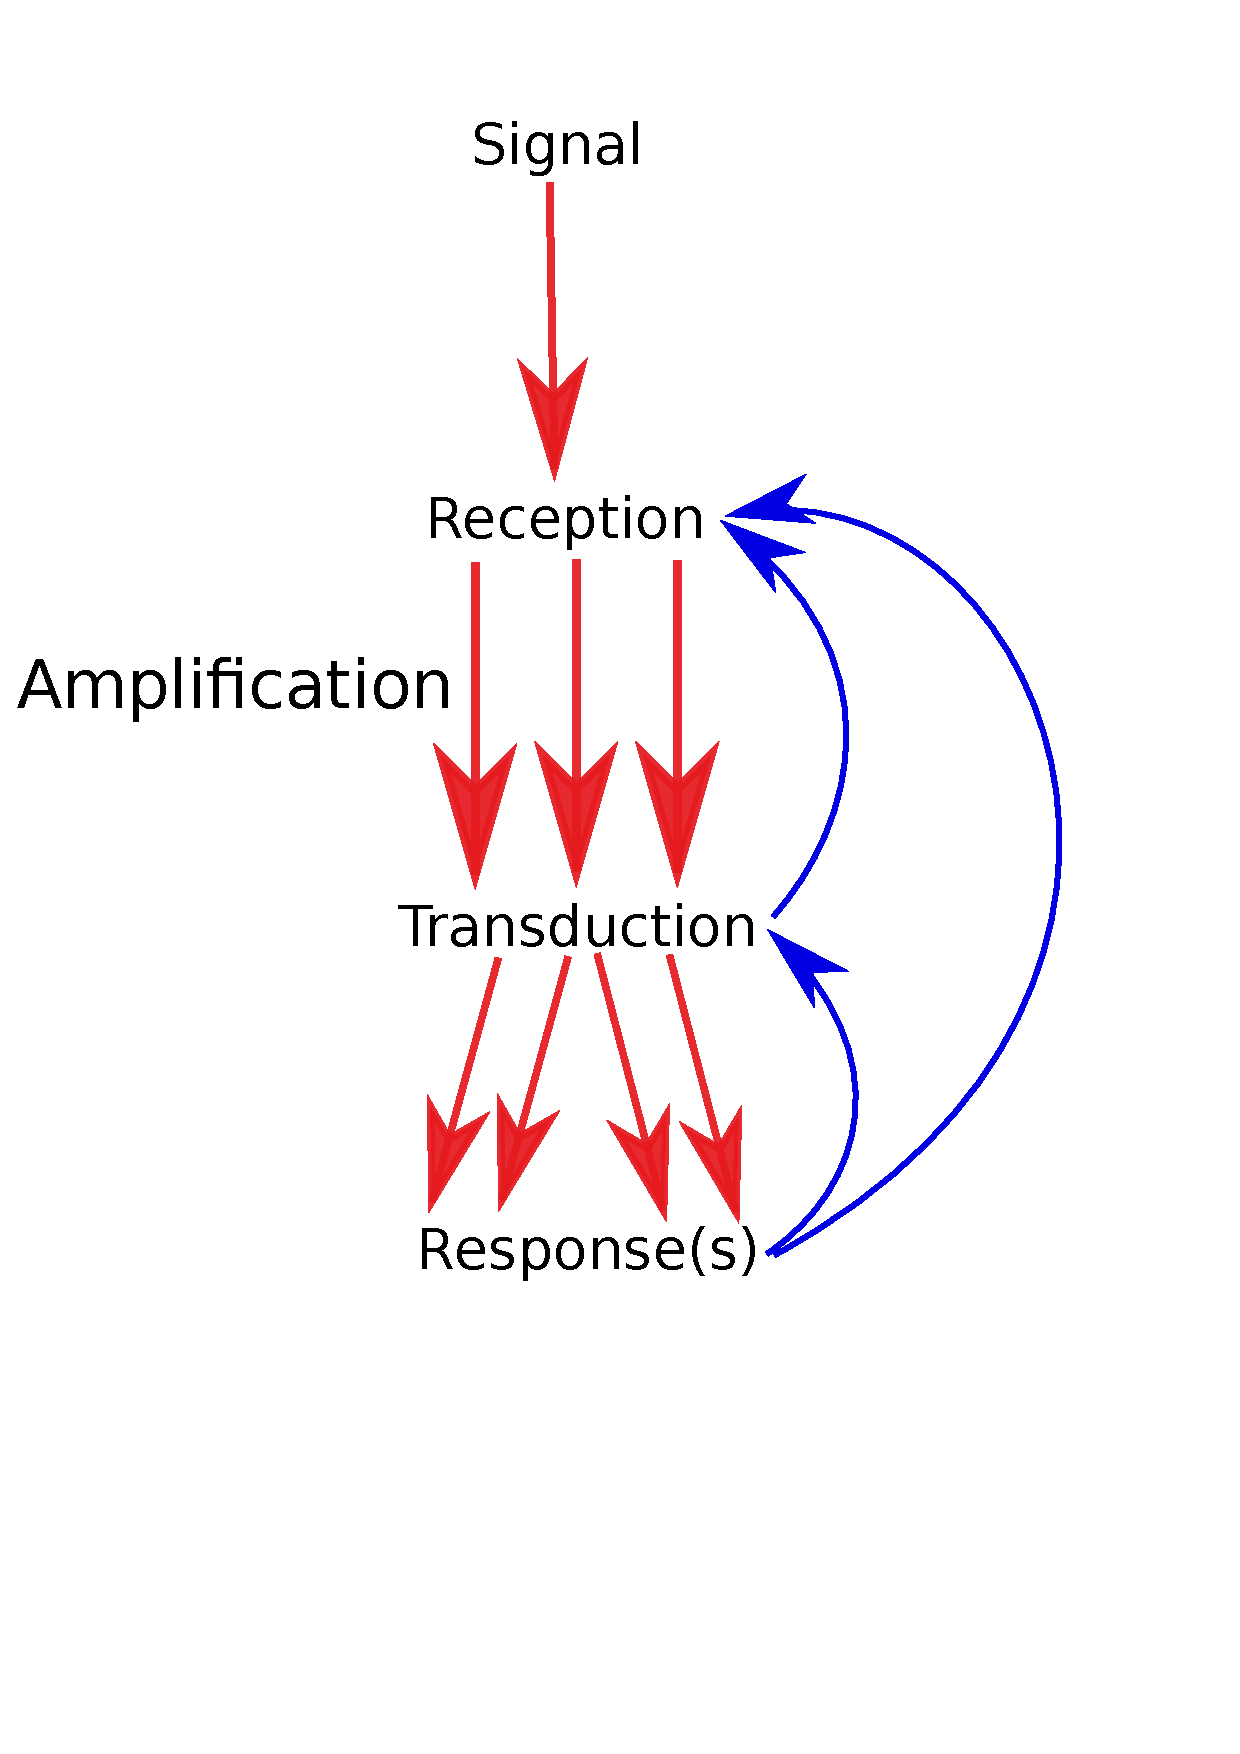
\includegraphics[width=0.5\textwidth]{./Bilder/signaltransduction.pdf}
\setlength{\abovecaptionskip}{-10ex}
\caption[Signal Transduction]{\textbf{Signal Transduction.} An environmental signal (e.g. hormone) interacts with a cellular component, most often a cell-surface receptor. The information that the signal has arrived is then converted into other chemical forms, or transduced. The signal is often amplified before introducing a response. Feedback pathways regulate the entire signaling process.\citep{Berg JM, Tymoczko JL, Stryer L. Biochemistry. 5th edition. New York: W H Freeman; 2002. Chapter 15, Signal-Transduction Pathways: An Introduction to Information Metabolism. Available from: https://www.ncbi.nlm.nih.gov/books/NBK21205/} }
%\setlength{\belowcaptionskip}{0pt} 
\label{fig:Fig.1.}
\end{figure}

\subsection*{Protein-Protein-Interaction}
In contrast to the gene regulatory interaction network the protein-protein interactions (PPIs) act directly among themselve. Thus the nodes in a network are the interacting proteins. Proteins interact by physical contacts(e.g. electrostatic forces) of high specificity. PPIs play a big role in electron transfer,signal transduction, transport across membranes and cell metabolism. A variety of techniques are known to detect PPIs. The most applicated ones are immuno-precipitations and the yeast two-hybrid approach. The two-hybrid assay is not a relieable indication that two proteins interact \textit{in vivo},because the two interacting proteins are overexpressed.Thus the interaction may not be present in the wild type cells where the concentrations may be significantly lower. For this reason additional information are included to figure out the occurence of true interaction, such as cellular localization and mRNA expression level. The underlying assumption is that true interactions are likelyto occur between proteinsinvolved in the same biological process, proteins found in the same cell compartment, and proteins whose mRNA are coexpressed.
For the identification of protein complexes affinity purification technique is used followed by mass spectrometry (MS) to sequence the proteins in the complexes. The detection of interactions of protein with DNA is done by chromatin immunoprecipitation (ChIP) in addition with expression microarrays, so-called ChIP on Chip approach. This method provide information about the interaction of transcription factors with DNA and the binding sites of transcription factors. Furthermore computational methods are included to predict the protein interactions by protein fusion and using phylogenetic analysis. Interaction networks of PPIs may depict how drug- protein interactions lead to toxic side effects.
%\citep{10.1371/journal.pcbi.1000807}
\citep{doi:10.1586/14789450.1.2.239}

\newpage
\section{Preprocessing}
%normalization and discretization of the data

\newpage
\section{Boolean Network}
%Define Boolean Network, decribe Definition, give an example
\textbf{Definition: Undirected Graph}\\
In general, an undirected graph $G=(V,E)$ is defined as a set of vertices $V$ describing the nodes of the system and a set of undirected edges $E = \{ (i,j)|i,j\in V\} $ that define a relationship between node $i$ and $j$.\\

This definition can be extended to obtain a notion of a directed graph:\\

\textbf{Definiton: Directed Graph}\\
A directed graph is an ordered pair $G=(V,A)$, defined as a set of vertices $V$ (nodes) and a set of directed edges $A$ (arcs). A set of directed edges $A=\{ (i,j)|\in V\} $ describes the flow of information in the system, where $(i,j)$ describes the flow from $i$ (tail)to $j$ (head). 



\section{Interaction Graph and State Transition Graph}


\textbf{Definition: Interaction Graph}\\
%Definition
%Describe Definition
%Give an example

\textbf{Definition: State transition Graph}\\
%Definition
%Describe Definition
%Give an example
Let $X$ be an \textit{n}-dimensional binary vector that represents the current state of the system. Each element $X_i\in X$ corresponds to the state ($0$ or $1$) of species $i$. A Boolean network defined by a set $F$ of \textit{n} Boolean functions. For every $f_i\in F$, such that $1\leq i\leq n,f_i(X(t))=X_i(t+1)$.\\ 

In other words,given a current state of thesystem $X(t),f_i$ determines the (binary) value of species $X_i$ at time $t+1$. Given a Boolean network $N$ on $n$ variables and an initial state $X(0)\in \lbrace 0,1\rbrace ^n$, the dynamics of the system can be simulated by repeatedly applying the Boolean functions and updating the "current" state.

\textbf{Definition: Boolean Regulatory Network}\\


\citep{10.1371/journal.pone.0066031}%An Evaluation of methods for inferring boolean Networks from time-series data
%---------------------------------------------------------------------------------------------------
A boolean regulatory network consists of nodes (vertices) representing the components of a system and the edges (links) representing  the interaction between the nodes. Each node can take two possible values of 1 (ON) or 0 (OFF). Depending on the input data this could mean, a gene is expressed or not, a transcription factor is active oder inactive, a molecular's concentration is above or below a certain threshold. The edges can be directed or undirected and show the orientation of masstransfer or information respectively. The future state of a node is determined by Boolean rule (function) shown in Figure 1.3. For instance the regulator $v1$ should be inactive such that the regulatee $v2*$ can be active. Here $v2*$ describes the future state of $v2$ \citep{SAADATPOUR20133}. 

\begin{figure}[H]
\centering
%\setlength{\abovecaptionskip}{0pt}
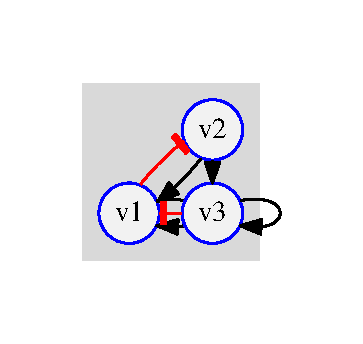
\includegraphics[width=0.4\textwidth]{./Bilder/example02_igraph}
\caption[Interaction Graph]{\textbf{Interaction Graph.} Shown is a selfinvented Interaction Graph constructed in PyBoolNet. The nodes $v1,v2,v3$ are denoted by blue circles, inhibitory arcs are red and activating arc are black. }
%\setlength{\belowcaptionskip}{0pt} 
\label{fig:Fig.3.}
\end{figure}

\begin{equation}
f(v_{1,2,3})= \begin{pmatrix}
 v_1      & \wedge v_2 & \wedge \neg v_2\\
 \neg v_1 &           & \\
         & v_2        &\wedge v_3
\end{pmatrix}
\end{equation} 



Beside the mathematical annotation, the boolean rule can be constructed with the operator AND,OR, NOT or they can be written as \& , ||, ! . The graph in Fig.1. is called the Interaction Graph. Updating the state of a node yield in a network several constellation of states for each node. Regarding the example in Fig.1 for each boolean rule in $f(v)$ all the possible combination of states every node can have is inserted. With $f(v)$ it is possible to determine the next possible state of each node to build an \textit{State Transition Graph}. 
The \textit{State Transition Graph (STG)} is a directed graph representing the dynamical behaviour of a Regulatory Graph. Nodes of this graph represent possible states of the model, assigning a value to each component. Arcs of the STG represent transitions from one state to another. It is an important network to analyze how data behaves over time, thus the most possible state of each component can be computed. But not every state of a component of a node is updated at the same time. Therefore the \textit{State Transition Graph} is either synchronous, updating all the node's states simultaneously, or asynchrounus, the node's states are updated based on their individual timesales\citep{Lee799}. \\\\\newline
Out of the \textit{Interaction Graph} of Fig.1. the synchronous and anysnchronous STG is computed and shown in Fig.2.\\

\begin{equation}
f(v) =  \begin{pmatrix}
 v_1\\
 v_2\\
 v_3
\end{pmatrix}
\textrm{, where }v_{1,2,3}\in\lbrace 0,1\rbrace
\end{equation}

\begin{figure}[h]
  \centering
 \begin{varwidth}{\linewidth}
    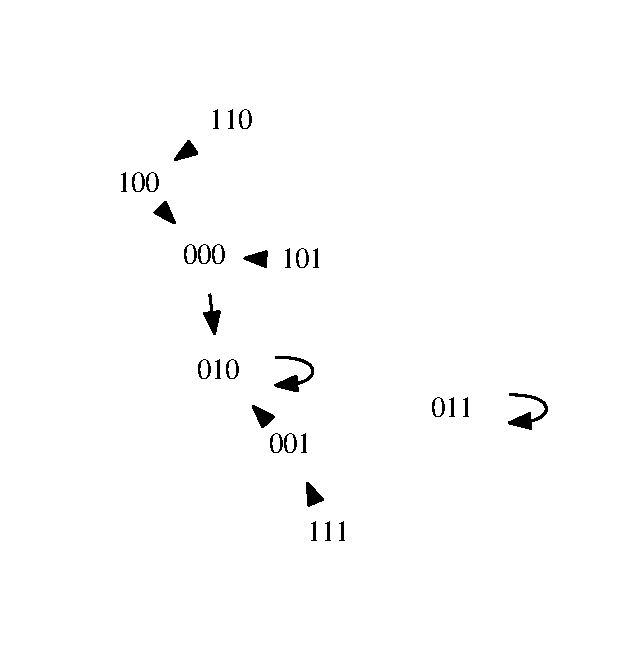
\includegraphics[scale=.5]{./Bilder/example01_synchron_stg}
  \end{varwidth} % ein Leerzeichen Abstand
  \begin{varwidth}{\linewidth}
    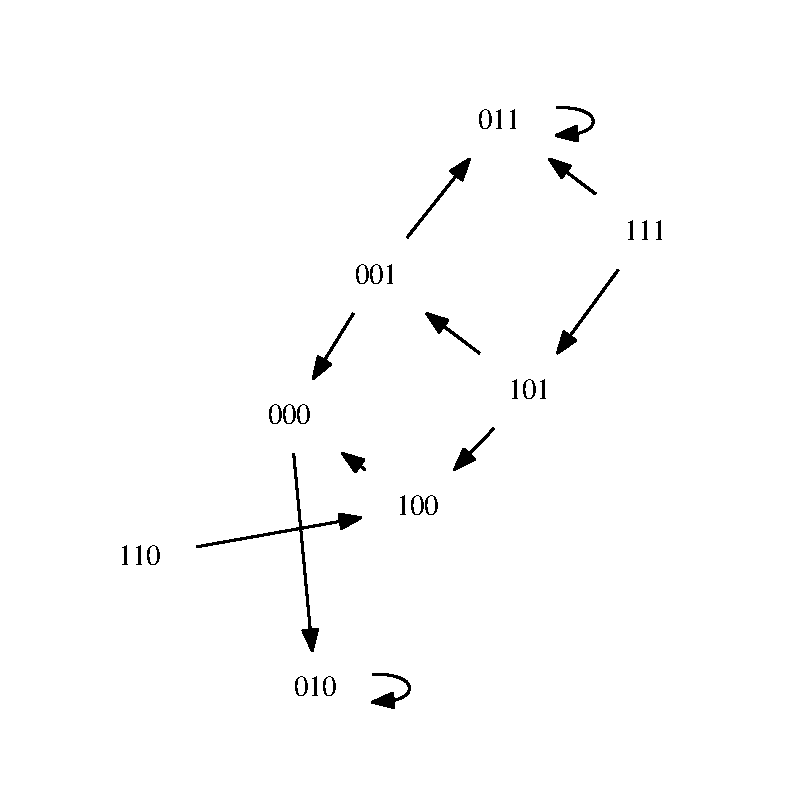
\includegraphics[scale=.4]{./Bilder/example01_asynchron_stg}
  \end{varwidth}
  \caption[Synchronous and Asynchronous State Transition Graph]{\textbf{Synchronous and Asynchronous State Transition Graph}. Left: Synchronous State Transition Graph; Right: Asynchronous State Transition Graph}
\label{fig:Fig.4.}
\end{figure}

%----Mathematische Definition von synchronen und asynchronen Update
\citep{REMY2008335}

\section{Network Evaluation}
%Define Accurancy, Precision, Recall, ROC, AUC


    \clearpage{\pagestyle{empty}\cleardoublepage}		% l�scht Kopfzeilen und Seitennummerierung von der letzten Seite eines Kapitels, sofern dort kein Text mehr steht
    \chapter{Materials and Methods}
\section{Data selection}
For a Boolean network inference the data of a platform so-called Dialogue on Reverse Engineering Assessment and Methods (DREAM) - Challenge is used. The DREAM-Challenge is a non-profit, collaborative community effort consisting of contributors from across the research spectrum of questions in biology and medicine. This organization was built in 2006 and publishes crowdsourcing challenges with transparent sharing of data, thus everyone can participate the challenge. The DREAM-Challenge has partnered with Sage Bionetworks, which provide the infrastructure by Sage Bionetworks Synapse platform to get access to the open collaborative data analysis. Overall the DREAM-Challenge is a helpful instrument to get real-life data, comparing results and interact with other researchers all over the world, while contribute solutions to biological and medical questions.
Two DREAM-Challenges appear useful for this work. The first is the DREAM5- Network Inference Challenge (DREAM5) and the second the HPN-DREAM brest cancer network inference challenge (DREAM8)\citep{DreamChalleneg Homepage}. 

\subsection{DREAM5}
Living cells are the product of gene expression programs involving regulated transcription of thousands of genes. Gene expression programs depend on recognition of specific promoter sequences by transcriptional regulatory proteins. How a collection of regulatory proteins associates with genes across a genome can be described as a transcriptional regulatory network. This map of the transcriptional regulatory network describes potential pathways bacteria cells (S.aureus, E.Coli, S. cerevisiae) can use to regulate global gene expression programs \citep{Lee799}.
The DREAM5-Challenge states the challenge to infere a complete (genome-scale) transcriptional regulatory network for four organisms: in silico, S.aureus, E.Coli, S.cerevisiae. 

%-----> Zeigen wie das in silico data set gemacht wurde?

The data is yielded by genechip experiments, where mRNA is extracted from the samples, then reversetranscriped into more stable cDNA (complementary DNA), which is fluorescent labeled. Afterwards the cDNA binds to the complementary bases on the chip. Thus the DNA composition can be detected and it can be recognized wether a gene is active or not by the information of its transcript.
Just the gene expression profiles for the in silico network were derived from another platform so-called GeneNetWeaver \citep{GeneNetWeaver}.

%\begin{table}[h]
%\centering
%\begin{tabular}{ccccc} 
%\hline
%Network & Organism & TranscFactors & Genes & Chips\\
%\hline
%Network 1 &	in silico &	195 &	1643 &	805\\
%Network 2 & S.aureus  & 99  &	2810 &	160\\
%Network 3 & E. coli   &	334 &	4511 &	805\\
%Network 4 & S. cerevisiae &	333 & 5950 & 536\\
%\hline
%\end{tabular}
%\captionof{table}{Overview}
%\label{table:Table 1}
%\end{table}\\


\begin{figure}
\centering
%\setlength{\abovecaptionskip}{0pt}
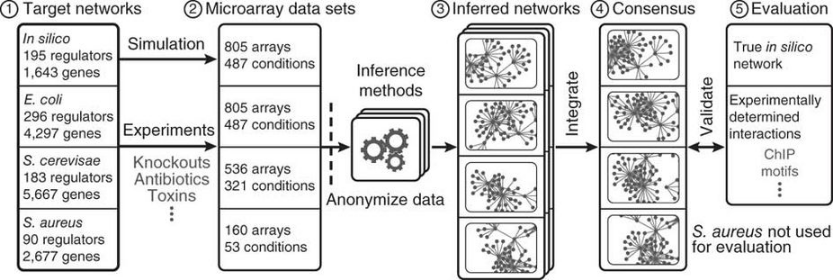
\includegraphics[width=0.8\textwidth]{./Bilder/assessment}
\caption[Interaction Graph]{\textbf{Assessment involved the following steps}Assessment involved the following steps }
%\setlength{\belowcaptionskip}{0pt} 
\label{fig:Fig.1.}
\end{figure}

In this challenge some experiments have pertubations in terms of gene deletion, overexpressed genes and  adding drugs to the system. Few experiments were done the same konfiguration several times. Some experiments are part of a time-series measurement and some are not,described in Figure 2.
For each network, a list of directed, unsigned edges had to be submitted ordered according to the participants confidence scores. 
The participants are given four microarray sets. In each set are three  tsv.-files  (tab-seperated values) with the gene expression data, chip-features and transcription factors.\\

\noindent\fbox{
    \parbox{\textwidth}{
\begin{flushleft}
\texttt{Network{\_}i{\_}\textbackslash{\_}expression\textbackslash data.tsv}\\
\texttt{Network{\_}i{\_}\textbackslash{\_}chip\textbackslash{\_}features.tsv}\\
\texttt{Network{\_}i{\_}\textbackslash{\_}transcription\textbackslash{\_}factors.tsv}\\
\end{flushleft}
    }
}


%where $i\in\lbrace 1,2,3,4\rbrace$

%\begin{center}
\begin{table}[H]
\scriptsize
\centering
\begin{tabularx}{\textwidth}{lllllllll} 
\hline\hline
Chip & Experiment &  Pertubations &  PertubationLevels &  Treatment &  DeletedGenes &  OverexpressedGenes &  Time &  Repeat\\
\hline \hline
1 & 1 &	NA & NA & NA & NA & NA & NA & 1\\\hline
2 &	1 &	NA & NA & NA & NA &	NA & NA & 2\\\hline
3 &	2 & NA & NA & NA & NA & NA & NA & 1\\\hline
4 &	2 &	P1 & 0.5 & NA & NA & NA & NA & 1\\\hline
5 &	2 &	P1 & 1.0 & NA & NA & NA & NA & 1\\\hline
6 &	3 &	NA & NA & NA & NA & NA & 0 & 1\\\hline
7 &	3 &	NA & NA & NA & NA & NA & 30 & 1\\\hline
8 &	3 &	NA & NA & NA & NA & NA & 60 & 1\\\hline
9 &	3 &	NA & NA & NA & G5 & NA & 30 & 1\\\hline
10 & 3 & NA & NA & NA & G5 & NA & 60 & 1\\\hline
11 & 4 & NA & NA & NA & G5,G8 & NA & NA & 1\\\hline
12 & 5 & P2,P3 & NA & NA & NA & G4 & NA & 1\\\hline
13 & 5 & P2,P3 & NA & 1 & NA & G4 & NA & 1\\
\hline
\end{tabularx}
\captionof{table}{Chip information}
\label{table:Table 2}
\end{table}
%\end{center}

The \texttt{Network{\_}i{\_}\textbackslash{\_}expression\textbackslash data.tsv} is a matrix where each entry $(i,j)$ describes the expression value of gene $j$ (column) in chip $i$ (row). The data has been normalized,such that the values are compareable across the experiments. For further computation it is necessary to dicretesize the data.

%-----> Normalization method
%-----> Discretisation method



The \texttt{Network{\_}i{\_}\textbackslash{\_}chip\textbackslash{\_}features.tsv} are shown in Table 2. where every row returns an identifier for the experiment that this chip is part of, then information about added drugs (Pertubations) and the dosage of the drugs (Pertubation Level). The Treatment shows the type of treatment used to apply the pertubations. Additionally are 2 columns showing Deleted genes and Overexpressed genes. Time-scaled data is shown in the column Time and Repeat hepls to distinguish experimental replicants. Whenever an entry $NA$ occurs, none of these pertubation properties mentioned above have been done.
The file \texttt{Network{\_}i{\_}\textbackslash{\_}transcription\textbackslash{\_}factors.tsv} is a list of genes of the network that are potential transcription factors for the network i (where $i\in \rbrace 1,2,3,4\lbrace$). Only these transcription factors should be included as regulators in the submitted network.\\

The predicted network is submitted with no more than 100.000 regulatory link predictions. These predictions are ordered from the most reliable to the last reliable prediction and put in a tab-seperated column format.

%----> Example of the submission

Organism specific gold standards containing the known transcription factor to target gene (transcription factor-target gene) interactions (= true positives) were compiled for assessing the participating approaches. All transcription factor-target gene pairs that are not part of the gold standards are seen as negatives, although, as the gold standards are based on incomplete knowledge, they might contain yet unknown true interactions. For evaluation of the predicted networks the AUPR (Area Under Precision Recall), AUROC (Area Under Receiver Operating Characteristic) and an ove-all accuracy was used.

%---->  Explain AUPR and AUROC and overall accuracy?




\subsection{DREAM8}





\subsection{Comparision DREAM 5 vs. DREAM8}
The DREAM5 challenge deals with high-throushput data of a microarray set in contratst to the DREAM8 challenge which deals with PPIs (protein-protein interactions). But in the DREAM5 challenge time-series data is mixed with data where no time was captured. Furthermore the experiments in DREAM5 contain a lot of additional information (pertubations by drug, gene deletion,overexpression of genes,replicate experiments) which is not needed in this thesis. 

\subsection*{Preprocessing of the data}
\citep{DISCRETIZATION}
%Discretization by k-means binarization, Iterative k-means binerization.redundancy removal
\citep{10.1371/journal.pone.0066031}
%Inferencealgorithms of DREAM5,DREAM8
%Floatchart fuer eine Pipeline einfuegen, (Datensatz--> Normalisierung--> Diskretisierung---> Inferenz---> Accuracy der inferenz/ zeigen, dass ein Inferenzalgorithmus auf mehreren Datensaetzen funktioniert---> Ananlysen des Netzwerks mit PyBoolNet)

\section{PyBoolNet and BoolFilter}



    \clearpage{\pagestyle{empty}\cleardoublepage}
    \chapter{Pipeline and Results}
This chapter introduces a pipeline of the \textit{in silico} data set (Figure 3.3) and a pipeline for the DREAM8 Challenge data set (Figure 3.8) describing the processing of the data from discretization to inferring a network and finally scoring the predicted network against a gold standard network. The results of the \textit{in silico} data set are necessary to set the parameter for the DREAM8 Challenge pipeline. Both pipelines can be executed from the command line by a bash script and are available on Git: "github.com/ninakersten/Masterthesis". 

\section{Pipeline of the \textit{in silico} data set}

For both the sub-networks of \textit{E.coli} and the cell cycle network each set $F$ of transition function is executed to sets of continuous data ($S=\{ S_{1},S_{2},...,S_{n}\} $), which are generated with \textit{odefy}, a MATLAB- and Octave-compatible toolbox for the automated transformation of Boolean models into systems of ordinary differential equations %\citep{Krumsiek2010}
(Figure 3.3, Figure 3.1). With \textit{odefy} the number of sample points and the time interval for a data simulation can be determined. The time interval is set to a range of 1 to 50. The \textit{in silico} data sets are converted into the \textit{csv} format of the structure of the DREAM8 Challenge input data (Table 2.1) and for the discretization and learning step converted into a \textit{text} file format (Figure 3.1). Names of the species are anonymized by single characters depicted in the first header of a \textit{txt} file and original names are stored in a header below followed by the time course data set \textit{S}. Information about cell line, inhibitor and stimulus are neglected (Figure 3.1).

%\noindent See the following command :
%\begin{lstlisting}[language=bash]
%  $ bash insilico.sh 100 KM3 BESTFIT
%\end{lstlisting}

%bild zeigen, wie die Daten in dem file angeordnet sind.
\begin{figure}[H]
\captionsetup{width=0.9\linewidth}
\centering
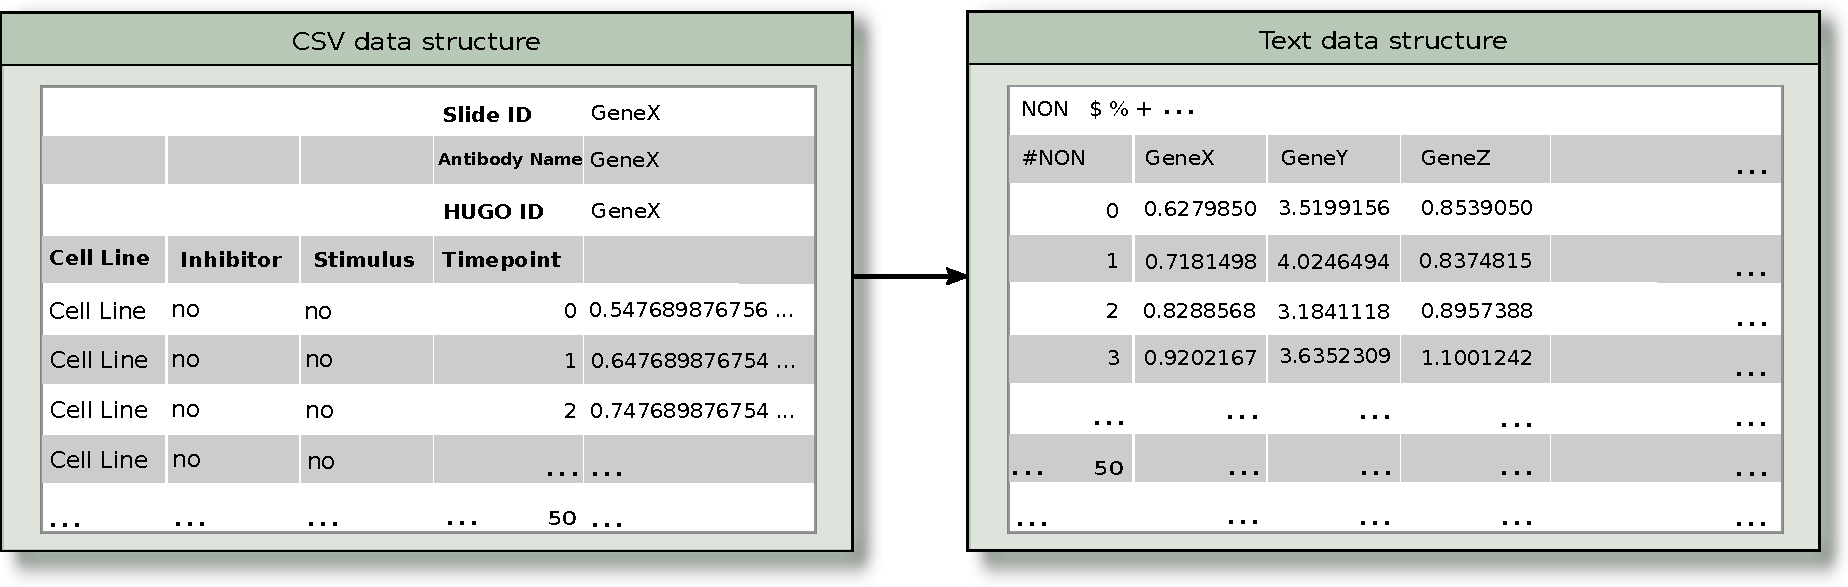
\includegraphics[width=1.0\textwidth]{./Bilder/CSV2TXT.pdf}
\caption[$CSV$ to $TXT$]{\textbf{$CSV$ to $TXT$:} Anonymized single character represent the species and information about cell line, inhibitor and stimulus is neglected. }
\label{fig:9}
\end{figure}

\newpage
After discretizing continuous time course data into a set of binary values ($B=bin(S)$, where $bin\in \{ $2-\textit{k-means}, iterative \textit{k-means}$\}$) redundant values are removed from this set. Boolean networks ($N=learn(B)$) are learned from this data by each inference algorithm ($learn\in \{$Best-Fit, Full-Fit, Reveal$\}$). A value for the minimal error $MinError$ is set, such that an inference algorithm runs i times (here: $i=5000$) until a network with an error ($Error(N,B)$) lower than the minimal error is achieved. 
%  Den Value für minimalen Error hier angeben= 10!!!!!
It is worthwhile to get an error of $0$, meaning the Boolean model describes the data perfectly. The amount of returned solutions is set to a value of $3$, such that in each inference process three solutions (resp. Boolean Networks) are inferred, all with an error lower than the minimal error. A single Boolean Network with the lowest error across all iterations is selected for further structural evaluation.
\subsection*{Inference settings}
For investigating the impact of the \textit{in-degree} in a network on the algorithms performance, sub-networks of \textit{E.coli} are processed by the iterative \textit{k-means} binarization algorithm with a cluster depth of $d=3$ in combination with Best-Fit, Full-Fit or REVEAL. The cluster depth with $d=3$ is selected due to previous research proving its reliability regarding the trade-off between simplicity and loss of information (e.g. oscillations).\\
\citep{Berestovsky.2013}
For assessing the dependence of an inference algorithm to the number of sample points, continuous data for the cell cycle is generated for $m\in\{ 50$, $100$, $150$, $200$, $250$, $300$, $350$, $400$ ,$450$, $500\}$. 
The whole set of inference algorithms only runs starting by 50 sample points. Complex systems, like a cell cycle are oscillating, thus a large number of sample points are needed to detect 'real' steady-states and achieve a sufficient Boolean network.\\

For measuring the impact of the clustering depth the cell cycle's continous data is generated with 100 sample points (similar to the abundance of sample points of $\sim 85$ in the DREAM8 Challenge) and inferred with a clustering depth of $d\in \{ 1,2,3,4,5,6,7,8,9,10\}$, where $d=1$ denote the two clusters \textit{k-means} binarization algorithm and from $d=2$ denote the iterative \textit{k-means} binarization algorithm. Table 3.1 shows a summarized overview of the settings for the \textit{in silico} pipeline.
%Hiernoch angeben, dass iterative k-means = d = 3
%und 2-k-means = d = 2
\begin{table}[H]
%\resizebox{\textwidth}{!}{
%{\tabcolsep=6pt%
\begin{center}
%\captionsetup{width=0.87\linewidth}
%\small
\scriptsize
\begin{tabular}{l|c|c|c}
\toprule 
Settings: Pipeline & \textit{in-degree} & sample points & cluster depth ($k$) \\
 \hline\hline
\# sample points & 100 & $[50:500]$ & 100 \\
\rowcolor{black!10} time interval & $[1:50]$ & $[1:50]$ & [1:50]\\
bin-method & $k=3$ & $k=3$ & $k \in [1,10]$\\
\rowcolor{black!10} REVEAL & \checkmark & \checkmark & \checkmark \\
Best-Fit & \checkmark & \checkmark & \checkmark \\
\rowcolor{black!10} Full-Fit & \checkmark & \checkmark & \checkmark \\
$MinError$ ($\epsilon$) & $0.6$ & $0.6$ &  $0.6$\\
\rowcolor{black!10} max. iteration ($i$)& 5000 & 5000 & 5000\\
solutions & 3 & 3 & 3 \\
\toprule
Network properties & & & \\
\hline\hline
\rowcolor{black!10} network source & $E.coli$ & Cell cycle & Cell cycle \\
\# networks & 45 & 10 & 10 \\
\rowcolor{black!10} max. \textit{in-degree} & $d\in [9:14]$ & 6 & 6 \\
\# nodes & $n\in [10:14]$ & 10 & 10 \\
\rowcolor{black!10} \# edges & $[10:126]$ & 35 & 35 \\
\bottomrule
\end{tabular}
\captionof{table}{Settings: Pipeline \textit{in silico} and network properties }
\end{center}
%}
\end{table}  

%!!!!!!MinError hier noch angeben!!!!!!

\subsection*{Prediction processing}

The predicted Boolean networks are converted (from \textit{.bnet}-format) into Interaction graphs (to a \textit{.sif}-format) by \textit{PyBoolNet} (Figure 3.2). Each interaction graph of a predicted network is scored against its gold standard interaction graph generated from the initial Boolean network with \textit{PyBoolNet}.\\
Hence, each line in a \textit{.sif}-file of an interaction graph represents an edge in a Boolean network (Figure 3.2). The edges of the gold standard and the prediction are compared resulting in a confusion matrix for computing precision, recall, accuracy, balanced accuracy and the Matthew correlation coefficient (Table 2.7).

\begin{figure}[H]
\centering
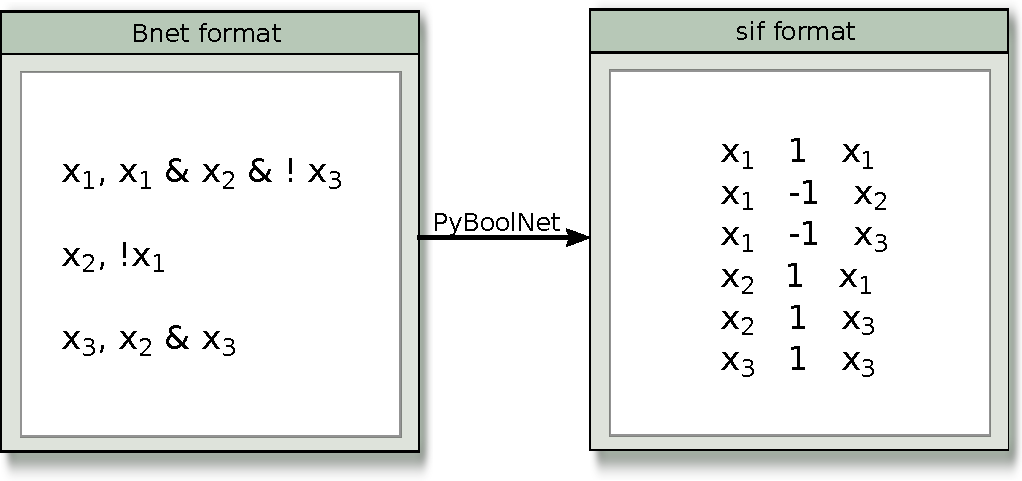
\includegraphics[width=0.7\textwidth]{./Bilder/bnet2sif.pdf}
\caption[Boolean Network to Interaction Graph]{\textbf{Boolean Network to Interaction Graph:} The predicted Boolean network $N$ (\textit{.bnet}-format) is converted into an interaction graph $IG$ (\textit{.sif}-format).}
\label{fig:9}
\end{figure}

 

\begin{figure}[H]
\centering
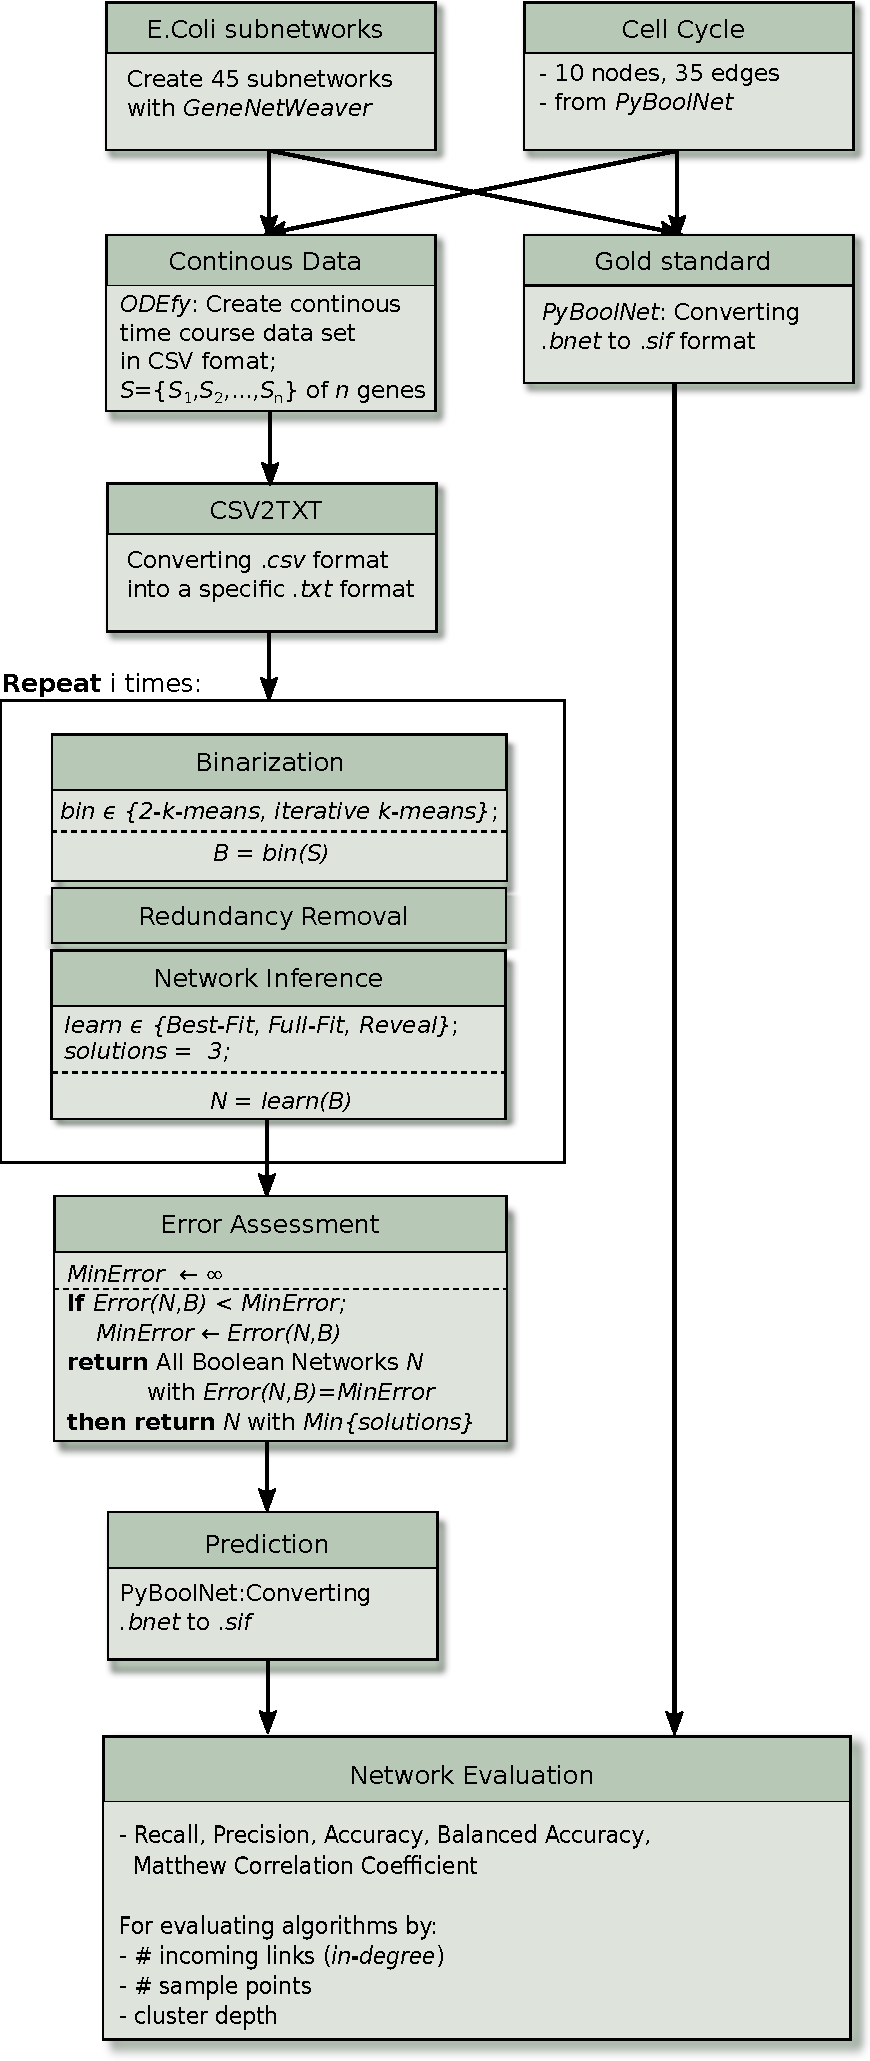
\includegraphics[width=0.55\textwidth]{./Bilder/pipeline_insilico.pdf}
\caption[Pipeline \textit{in silico}]{\textbf{Pipeline \textit{in silico}. }This pipeline shows the final setup for assessing the algorithms performance regarding the number of incoming links of nodes in a network, the number of sample points and the cluster depth for binarization.}
\label{fig:9}
\end{figure}



\section{Results and Discussion of the \textit{in silico} data set}
\subsection*{\textit{In-degree}}
Figure 3.4 shows 45 sub-networks of \textit{E.coli} grouped into nine categories, each containing five sub-networks with $n$ nodes; $n\in |V|$, where $|V|=\{10,11,12,13,14\}$. Each category on the x-axis depicts the \textit{in-degree} $k^{in}_i \in \{1,2,3,4,5,6,7, 8, 9\}$) of a set of nodes in a network. Thus, the inference algorithms Best-Fit, Full-Fit and REVEAL predict five networks in each category where the mean accuracy value is obtained by scoring each predicted interaction graph against a corresponding gold standard interaction graph, derived from the initial network $N'$ (Figure 3.3).\\
Starting with an \textit{in-degree} of $k^{in}_{1}=1$ the mean accuracy values of Best-Fit, Full-Fit and REVEAL are $\sim 0.854$, $\sim 0.844$ and $\sim 0.849$. With increasing \textit{in-degree} the mean accuracy value decreases for all three inference algorithms. Thus, with an \textit{in-degree} of $k^{in}_{9}=9$ the mean accuracy value for Best-Fit, Full-Fit and REVEAL are $\sim 0.399$, $\sim 0.407$ and $\sim 0.399$. None of the three inference algorithms show an outstanding significantly higher or lower mean accuracy. Hence, on average about $\sim 85,2\% $ of relevant links are predicted correctly by all three inference algorithms when the \textit{in-degree} is $k^{in}_{1}=1$ and an average of about $\sim 40,2\% $ of relevant links are predicted correctly by an \textit{in-degree} of $k^{in}_{9}=9$.

\begin{figure}[H]
\captionsetup{width=0.9\linewidth}
\centering
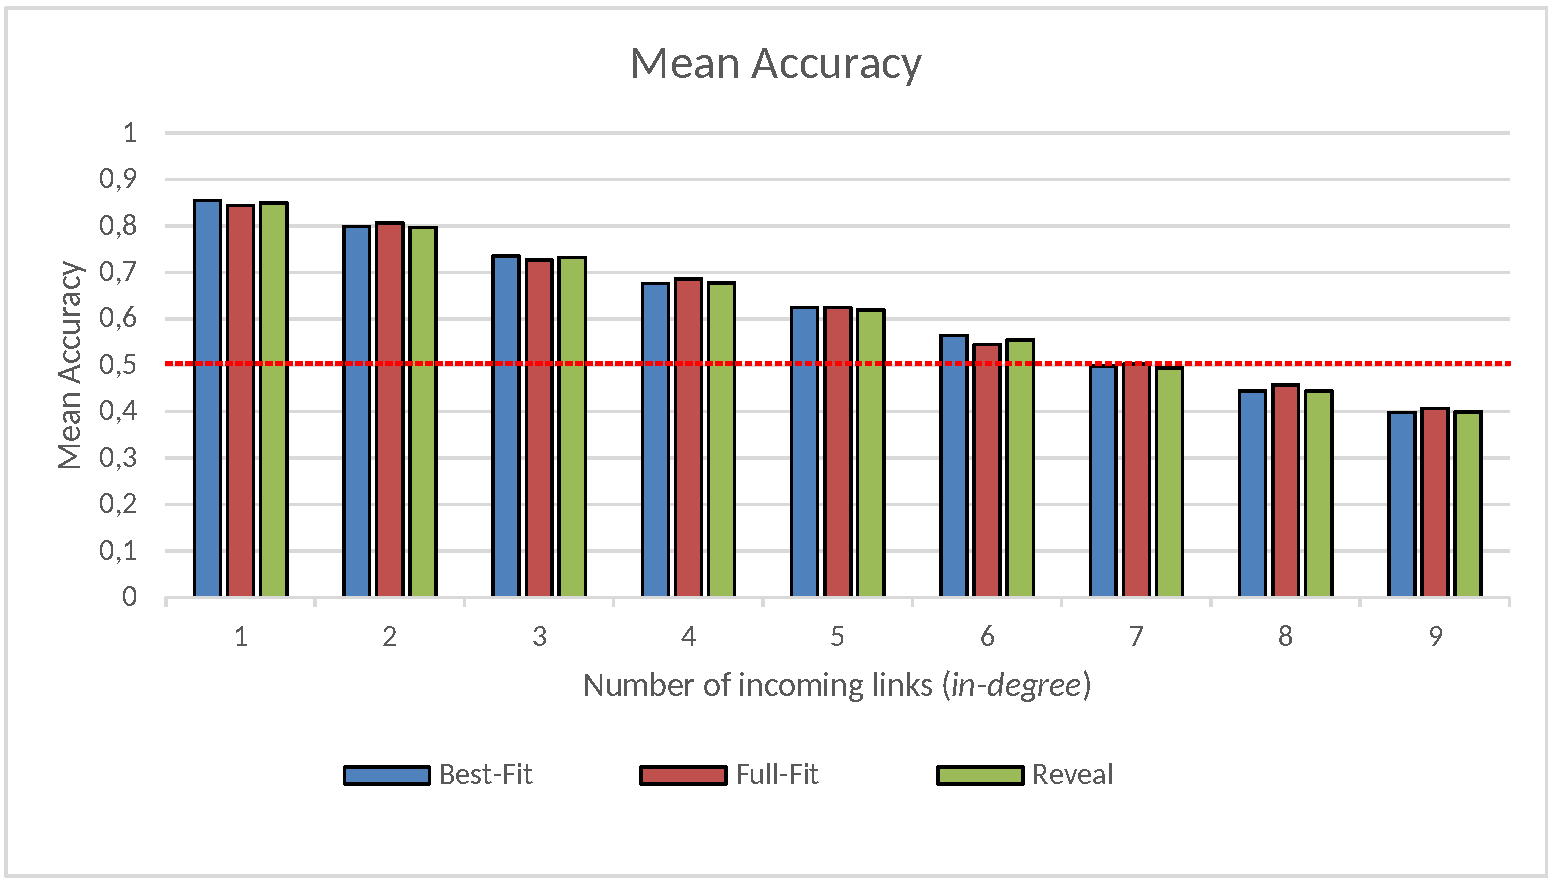
\includegraphics[width=0.9\textwidth]{./Bilder/Scoring/insilico/1_Indegree_Runtime/MeanAcc_indegree.pdf}
\caption[\textit{In-degree}:Mean Accuracy]{\textbf{\textit{In-degree}:Mean Accuracy.} Sub-networks of \textit{E.coli} are grouped into nine groups definded by the \textit{in-degree} of nodes in each sub-network. With increasing \textit{in-degree} the mean accuracy of all three inference algorithms decreases.}
\label{fig:}
\end{figure}

Thus the more nodes occur with a high \textit{in-degree} the more complex is the system and the worse the inference algorithm is able to detect the whole information. This observation captures the observation of Shohang Barman and Yung-Keun Kwon \citep{Barman.2017} who state that the number of incoming links represent the degree of complexity of the inference problem. They introduced a novel mutual information-based Boolean network inference (MIBNI) method and tested its structural and dynamic performance. Therefore, about $\sim 300$ sub-networks of \textit{E.coli} of different network sizes ($|V| = 10,20,$...$,100$) were randomly generated by $GeneNetWeaver$ and nodes of these networks were grouped by their \textit{in-degree}. Their new method yielded a slightly better performance in contrast to Best-Fit and REVEAL. Nevertheless, with incresing number of incoming links the mean accuracy decreases for all measured inference algorithms assessed in this article, too.

%Diskussion:
%- The more complex a system is (nodes have high in-degree) the more challenging it is to predict whole set dertiming a nodes state.

%\newpage
\subsection*{Number of sample points}
Continuous data sets of the mammilian cell cycle network are generated with different number of sample points $m\in \{50,100,150,200,250,300,350,400,450,500\}$ and the predicted interaction graph is scored against the interaction graph of a gold standard cell cycle interaction graph derived from the initial network (Figure 3.3).\\
In Figure 3.5 (a) recall values of Best-Fit, Full-Fit and REVEAL are ranging between $0$ (REVEAL) and $\sim 0.231$ (Best-Fit). The values fluctuate across the number of sample points for each of the three inference algorithms and regarding the overall mean recall, about $\sim 9.49\%$ of relevant links ($TP$ and $FN$) are predicted. \\
Taking the precison in Figure 3.5 (b) of Best-Fit, Full-Fit and REVEAL into account the values fluctuate among the increasing number of sample points, too. Here, values range from $0$ (REVEAL) to $\sim 0.428$ (Best-Fit). 
The mean precision value of Best-Fit is $\sim 0.236$ and for Full-Fit is $\sim 0.252$ and for REVEAL is $\sim 0.219$. \\
Thus, averaging across Best-Fit, Full-Fit and REVEAL about $\sim 23,6\% $ of the predicted links are predicted correctly.

\begin{figure}[H]
\captionsetup{width=0.9\linewidth}
\centering
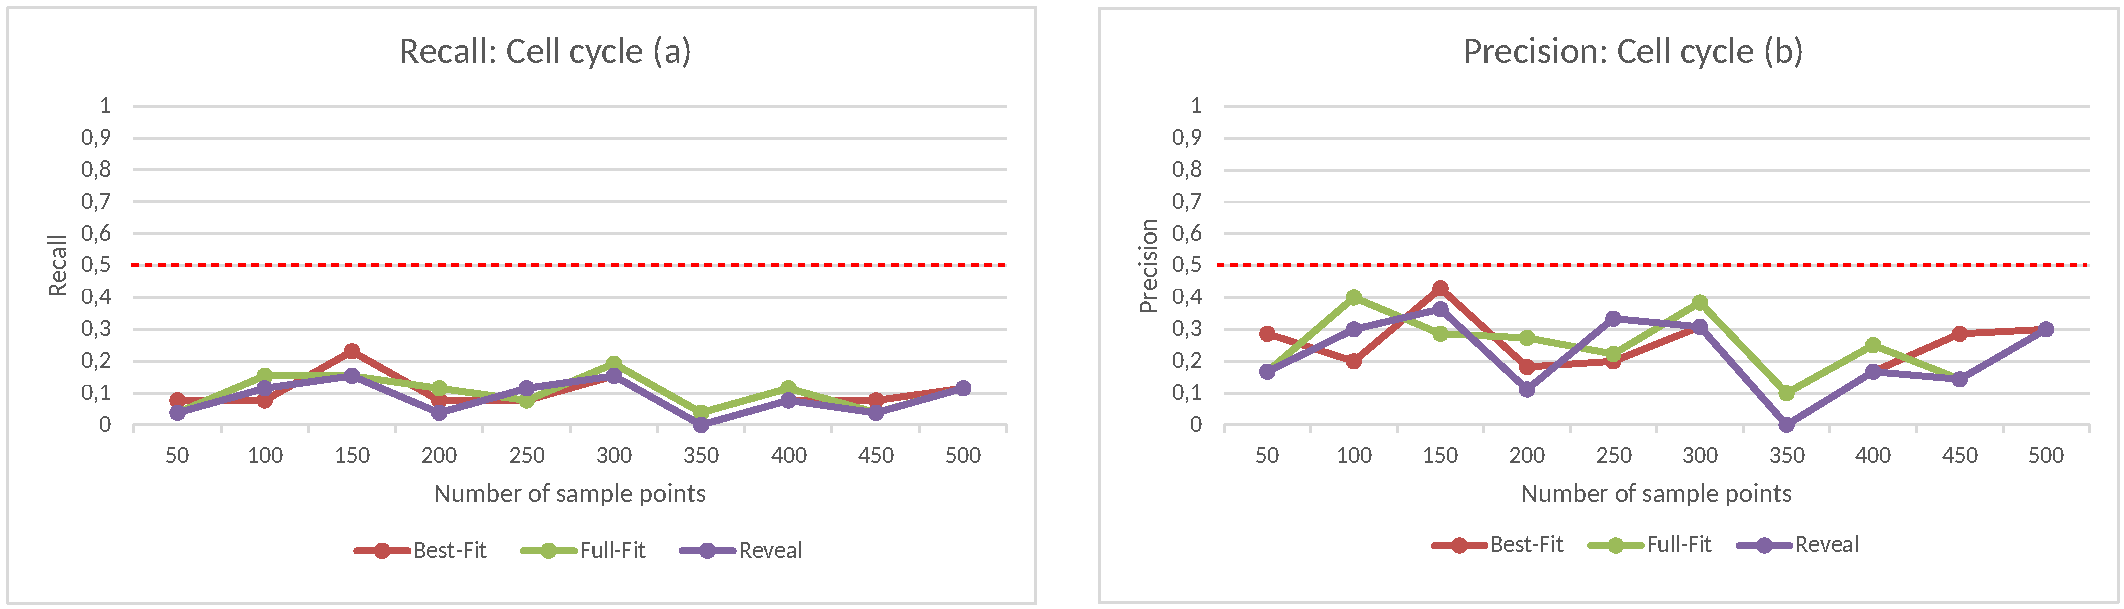
\includegraphics[width=1.0\textwidth]{./Bilder/Scoring/insilico/2_cellcycle_measurements/RecPrec.pdf}
\caption[Precision and Recall: Number of sample points]{\textbf{Number of sample points.} (a) Recall for Best-Fit, Full-Fit and REVEAL; (b) Precision for Best-Fit, Full-Fit, REVEAL}
\label{fig:}
\end{figure}
\newpage
Fluctuations across the increasing number of sample points in Figure 3.5 may be a result of the oscillating property of the cell cycle system, which is not captured in each network. The number of false negative predicted links is tremendeously high in constrast to the number of true positive predicted links for all inference algorithms, which explaines the recall. While precision is taking the true positive and false positive predicted links into account, which are not that highly class im-balanced like the classes for the recall are.\\

For this reason the balanced accuracy is considered (Figure 3.6). Here, the class imbalance is relativized, such that all three inference algorithms range around a value of $\sim 0.5$ among the increasing number of sample points. This means, each inference algorithm predicts the links in a network rather randomly. 

\begin{figure}[H]
\captionsetup{width=0.9\linewidth}
\centering
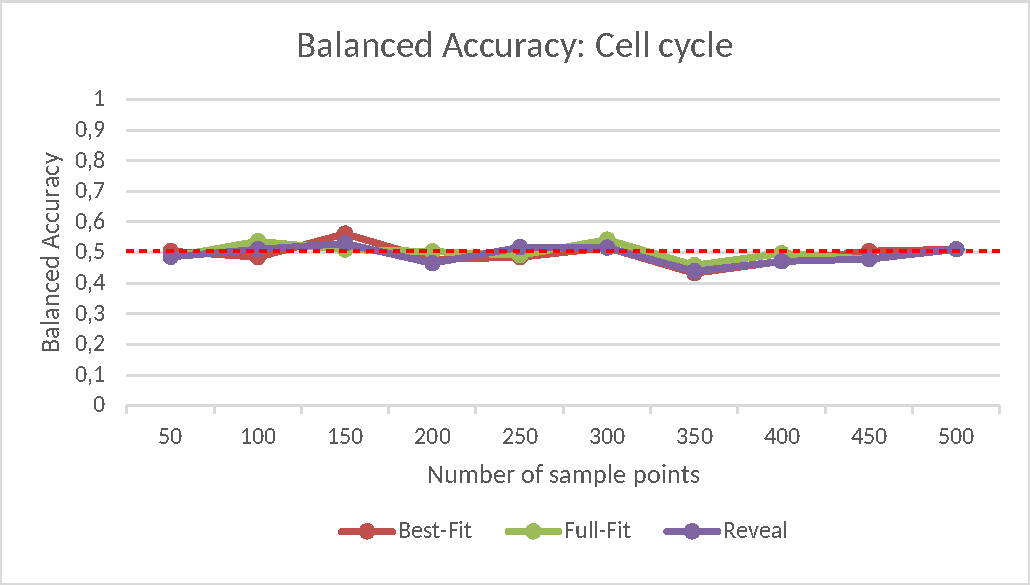
\includegraphics[width=0.9\textwidth]{./Bilder/Scoring/insilico/2_cellcycle_measurements/Bacc.pdf}
\caption[Balanced Accuracy: Number of sample points]{\textbf{Balanced Accuracy: Number of sample points.}}
\label{fig:}
\end{figure}

Regarding recall, precision and balanced accuracy in this setting context it is observed that the number of sample points has no significant impact on the inference algorithms' performance.\\
The cell cycle is with 35 links a highly interconnected network and due to its' oscillating property quite challenging to infer.
Thus, taking prior knowledge from literature into account it is important to mention, that this observation is not true for less complex networks of smaller size \citep{Berestovsky.2013}. %\citep{ "Boolean network inference from time series data incorporating prior biological knowledge" Haider and Pal BMC Genomics 2012, 13(Suppl 6):S9 http://www.biomedcentral.com/1471-2164/13/S6/S9}



%Diskussion:
%- inference algorithms are stable across the number of sample points
%- Precision: Fluctutation because of oscillating system of the cell cycle, thus in combination with the binarization method (KM=3) sometimes steady-states are detected well, low Error, and sometimes not
%-The more nodes are in a system, the more time points are needed to capture dynamics of a system
%- Meets observation of \citep{TS2B-Paper}, where with increasing number of nodes and thus, increasing complexity the number of sample point have to increase, such that tru dynamics can be captured (find a network below minError). e.g. In \textit{Jak-Stat} signal transduction pathway with 5 nodes (pJak2, pEpoR, pStat5, CIS, Socs3) with only 14 timepoints, no oscillations, but for a system of cell cycle with 10 nodes at least 30 time points are needed for Best-Fit and Full-Fit and $\sim 50$ time points are needed for REVEAL.
% Recall: Nur 10%, weil: MinError sehr groß gewählt wurde.
% Precision: Fluctering, weil cell cycle oscilating system. Binarization algorithm capture dynamics sometimes well, sometimes not. Wert gut, weil TN stark den tp überwiegen. Recall schlecht, weil FN genauso hoch wie TN und TP sehr wenig.
\newpage
\subsection*{Cluster depth}
In Figure 3.7 the cluster depth $d$ is increased from $d=1$, which represents the two clusters \textit{k-means} binarization algorithm and from $d=2$ to $d=10$ describing the cluster depth of the iterative \textit{k-means} binarization algorithm. In (a) the Matthew correlation coefficient starts with the highest value of $\sim 0.258$ for REVEAL for $d=1$ followed by Full-Fit with a value of $\sim 0.106$ and Best-Fit with $\sim 0.106$. Proceeding with $d=3$ Best-Fit stands out with a value of $\sim 0.258$ whereas Full-Fit and REVEAL range around a value of $0$. With increasing cluster depth the performance of all three inference algorithms approximates around a mean value of $\sim 0.048$.\\
In comparison with balanced accuracy in (c) when $d=3$ Best-Fit perfoms the best with a value of $0.588$ as well. Increasing the cluster depth yields an approximation of all inference algorithms around a mean value of $\sim 0.516$.\\
In (b) Best-Fit yields the best performance with a precision value of $0.6$ and  $d=3$. The value highly fluctuates until $d=5$ and approximates from $d=6$ to a precision value of $\sim 0.287$. Regarding the recall in (d) none of the inference methods is significantly outstanding. Taking the mean recall approximatly $\sim 12,3\% $ of relevant links are predicted by the methods. While $\sim 28,7\% $ of predicted links are correctly predicted.

%Overfitting:\citep{ https://doi.org/10.1371/journal.pone.0162259}

%Regarding the precision (Figure 3.7 (b)) 
\begin{figure}[H]
\captionsetup{width=1.0\linewidth}
\centering
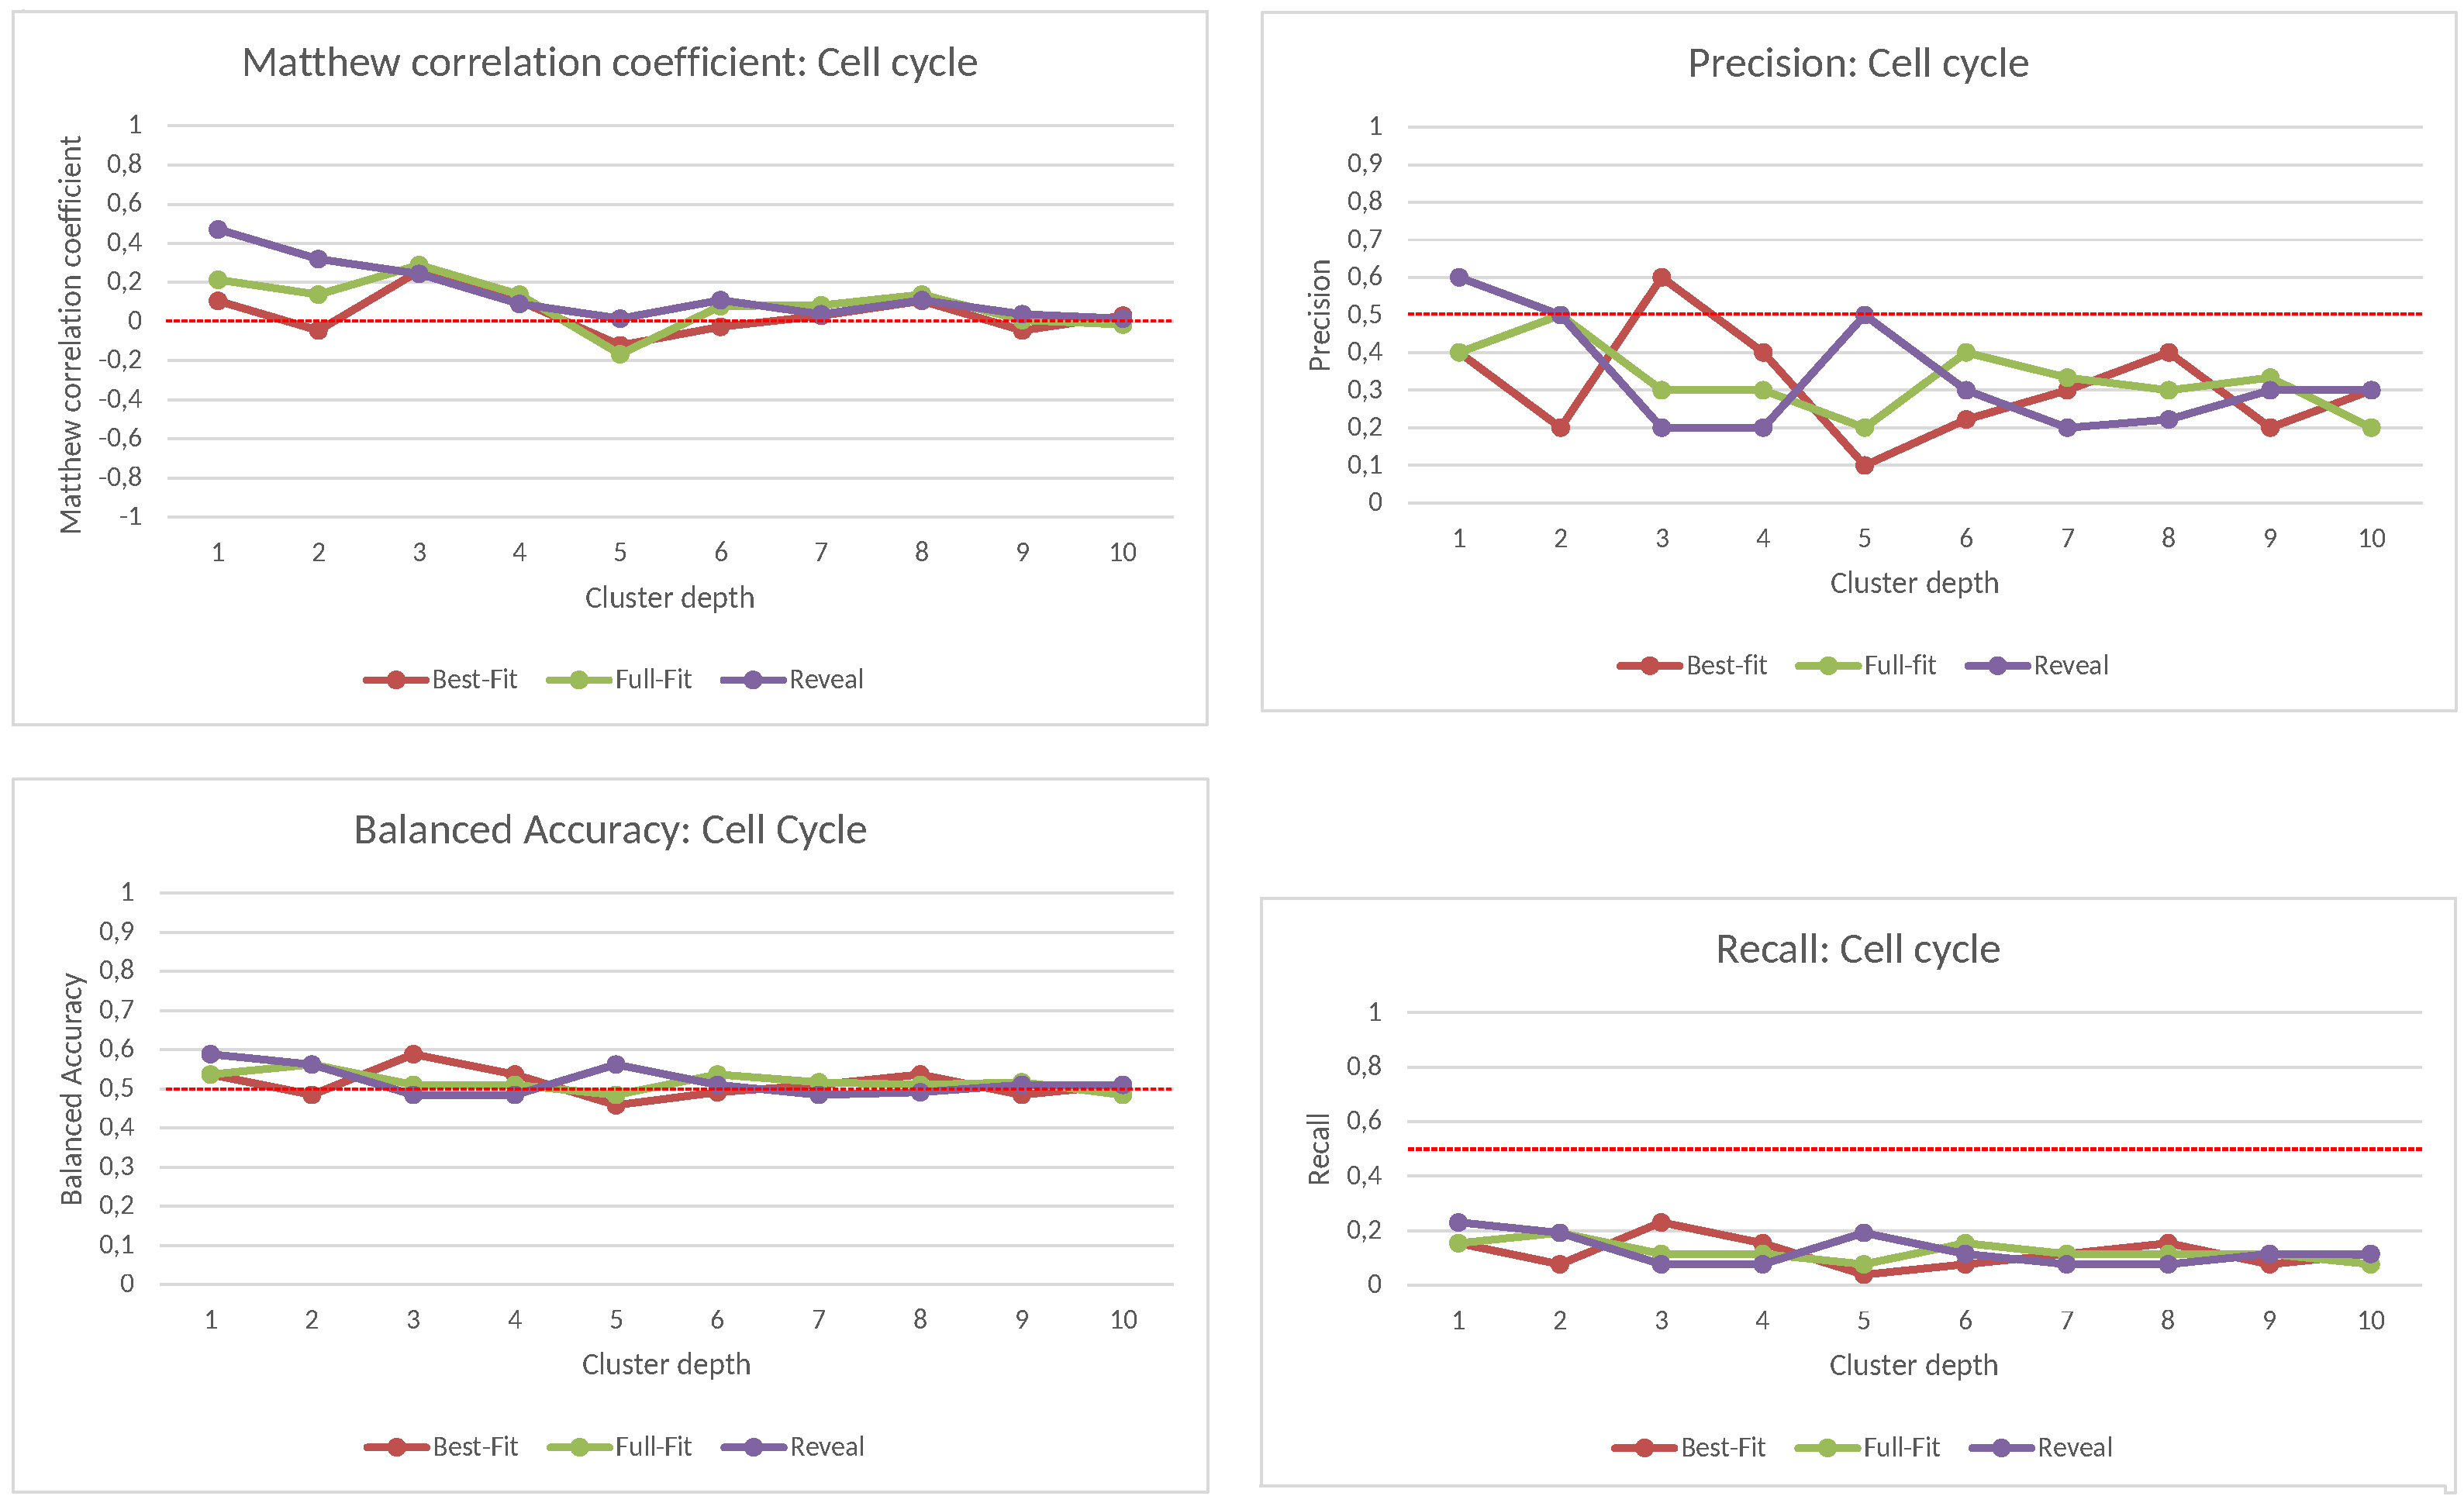
\includegraphics[width=1.0\textwidth]{./Bilder/Scoring/insilico/3_cellcycle_clusterdepth/insilico3.pdf}
\caption[Performance considering cluster depth \textit{d}]{Performance considering cluster depth \textit{d}}
\label{fig:7}
\end{figure}

Results of the performance measurement in dependence on the number of sample points are similar to the results of performance measurement in dependence on the cluster depth regarding fluctuations in precision, Best-Fit is performing the best across precision and recall and balanced accuracy and Matthew-correlation-coefficient show no outstanding performance of a method. Futhermore, regarding the runtime performance is REVEAL computuationally expensive (Figure 2.2) and therefore not an appropriate method for big real-life data network inference. Taking prior knowledge from literature into account then Best-Fit in combination with the iterative \textit{k-means} binarization algorithm captures the structural and dynamic complexity in a system the best \citep{Berestovsky.2013}.
For these reasons, this combination is applied to the real-life data set of the DREAM8-Challenge described in the next section.
%%%Wie kann man die Fluktuationen erklären????
%Diskussion:
%- MCC+BACC: TN und FN werte sind deutlich höher, daher reguliert es diese werte.
% Recall: zeigt dadurch eher, dass gerademal mean recall 9,5% der relevanten elements are selected sind und durch precision weiß, man, dass mean precision: 23,6% der selected elements sorrect sind.
%Hohe Fluktuation bei Precision: Higly oscillating system.
%\newpage
\section{Pipeline of the DREAM8 Challenge data set}
\begin{figure}[!h]
\centering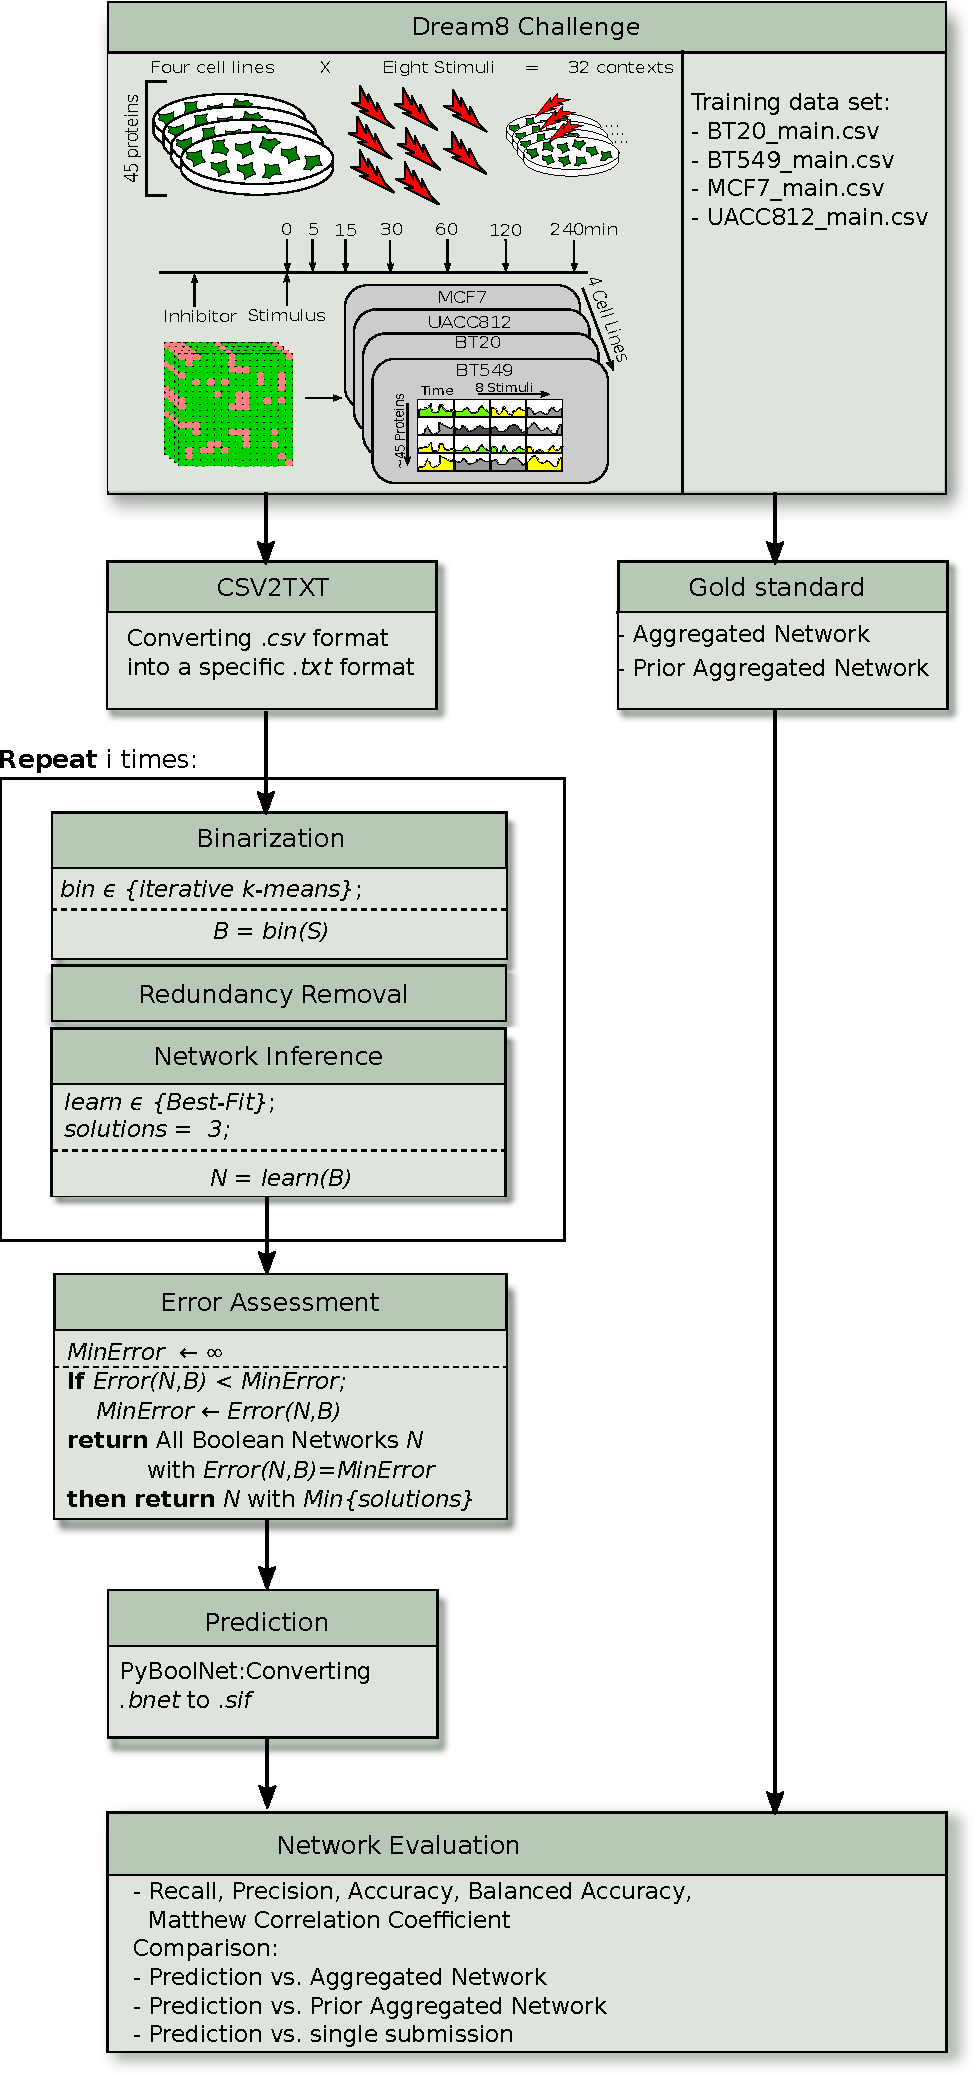
\includegraphics[width=0.6\textwidth]{./Bilder/pipeline_dream8.pdf}
\caption[Pipeline DREAM8-Challenge]{\textbf{Pipeline DREAM8-Challenge. }This pipeline shows the final setup for the DREAM8-Challenge input data. Settings are selected by previous investigation of the \textit{in silico} data set and prior knowledge from literature.}
\label{fig:9}
\end{figure}

%Threshold: Wenn ich mehrere solutions habe, dann edge score berechenen über die Häufigeit von auftretenden Kanten, dann threshold verschieben, sodass von wenig bis viele tp sich ergeben = AUROC / = AUPR (Wegen runtime nicht gemacht,aber ich dann es ja für nur 3 runs zeigen?)


%Create 32 data set from training data -> txt. file
In this section it is shown in which way the \textit{in silico} pipeline is validated, such that the DREAM8-Challenge data set can be processed, resulting in a DREAM8-Challenge pipeline depicted in Figure 3.8.\\ 
This pipeline starts with the 'main' training data set of the DREAM8-Challenge, which is converted into a \textit{txt} file format (Table 2.1, Figure 3.1) by splitting each data set of a cell line into eight text files depending on each stimulus. Each of the resulting 32 \textit{text}-files contain about $\sim 85$ sample points and about $\sim 45$ antibody names.

\subsection*{Setting selection}
%Quelle: TS2B Paper mit KM3 Empfehlung
%The python implementation of the inference algorithms is validated, such that a network up to 50 nodes can be inferred and the 
%Network inference: KM3+Best-Fit
The higher the \textit{in-degree} of each node (Figue 3.4) and the abundance of nodes in a network (Figure 2.2) the higher is the complexity in a system and hence, the higher is the computational cost of an inference algorithm \citep{Barman.2017}. 
The aim of the \textit{in silico} pipeline is to investigate which parameter has a major influence on the algorithms performance, such that the best performing algorithm can be selected for the DREAM8-Challenge data set.\\
As mentioned in 2.1 technical requirements limit (8 RAM and a Core i5 processor) the application of REVEAL to the DREAM8-Challenge data set resulting an infeasible task (Figure 2.2). This observation is confirmed by Shohang Barman and Yung-Keun Kwon \citep{Barman.2017} who state that mutual information based approaches like REVEAL are computationally expensive, because they are implemented to compute the exact mututal information values over all possible combination of nodes. Therefore, REVEAL is not considered in this pipeline.\\\\

Furthermore, results of the \textit{in silico} pipeline regarding the choice of abundance of sample points (Figure 3.6) and cluster depth (Figure 3.7 (c)) show no significant influence on the algorithms' performance. An increasing \textit{in-degree} (Figure 3.7 ) shows an decreasing performance for all three algorithms, such that no algorithm can be excluded by this investigation either.\\\\
Thus, results regarding error assessment of Best-Fit, Full-Fit and REVEAL in combination with two cluster \textit{k-means} binarization algorithm and iterative \textit{k-means} binarization algorithm of Natalie Berestovsky and Luay Nakhleh are taken into account. In this paper based on minimal error, convergence and uniqueness the recommended combination of Best-Fit with the iterative \textit{k-means} algorithm (with $d=3$) for complex systems is applied to the DREAM8 Challenge data set.\\\\%Tabelle in das supplementary,wo gezeigt wird wie gut die performance ist?
As in the \textit{in silico} pipeline the minimal error is set to a value of ????? and maximally runs 5000 times by returning 3 networks and selecting the solution with the lowest error. Predicted Boolean networks (in \textit{bnet}-format (Figure 3.2)) are converted into an interaction graph (in \textit{sif}-format (Figure 3.2)) and scored against two aggregated networks
each representing an aggregated network and an aggregated prior network each representing a gold standard.\\\\ 

For simplification of notation the prediction is defined by the set of networks predicted by the DREAM8-Challenge pipeline with the inference algorithm Best-Fit and the iterative \textit{k-means} binarization algorithm with $d=3$.


\subsection*{Gold standard and Evaluation selection}
Since gold standard networks are often based on prior knowledge from literature, learning novel connections in a network, such that specific biological systems can be truly mimicked is restricted \citep{Hill.2016}. Therefore, the DREAM8-Challenge did not provide a gold standard to the participants. Thus, a provided test data set was used as an abstracted representation of a gold standard to asses the algorithms' performance resulting in prior knowledge independent networks. \\
%Additionally an \textit{in silico} data set covering main characteristics of the experimental setting, but without batch effects, is provided by the challenge. This \textit{in silico} data set is a tool for assessing the performance of an algorithm in an idealized setting. Hence, the performance of an algorithm excluding pertubational effects can be assessed.
%The \textit{in silico} data set is generated from a non-linear ordinary differential equations (ODE) model of the ERBB signalling pathway (ERBB:family of proteins containing four receptor tyrosine kinases, structurally related to the epidermal growth factor receptor (EGFR)). Nevertheless pre-existing biological knowledge was included by several participants and seemed to be broadly beneficial.\\
%Warum beneficial? Zeigen, dass die performance der gruppen mit prior knowledge nicht signifikant schlechter war als bei gruppen ohne

%Evaluation in the DREAM8-Challenge
Due to varying strategies of evaluating predictions, e.g. choice of the scoring metric and implementation strategy, it is quite challenging to compare the resulting performances between the participants reliably. For this reason the DREAM8-Challenge provides a standard scoring tool: 'DREAMTools' python package \citep{Cokelaer.2015}.\\
This tool needs as input a \textit{sif}-file and an \textit{eda}-file, while an \textit{eda} (electronic design automation) contains information of edge occurrences in a network like in a \textit{sif}-file and additionally a confidence score for each edge. A confidence score (resp. edge weight) describes the probabilty of an edge being existent or not \citep{authornamenotavailable.}.\\ 

DREAMTools compares the confidence scores of a predicted network against confidence scores of a gold standard network returning values of the Area Under the Receiver Operating Characteristic curve (AUROC) and the Area Under the Precision Recall Curve (AUPR) \citep{Cokelaer.2015} \citep{Hill.2016}. Both evaluation metrics are commonly used when there is an imbalance between the number of positives and negatives in the gold standard \citep{Davis.2006}.
For further details regarding definition and application of these metrics the reader is referred to section A.1.'DREAM8-Challenge scoring priciples'. In subchallenge SC1A of the DREAM8-Challenge each participating group was ranked by their scoring results, revealing which inference performs the best \citep{authornamenotavailable}.\\\\

In contrast to the DREAM8-Challenge this work makes use of an aggregated network and an aggregated prior network each representing a gold standard. These networks were submitted after finishing the challenge in 2016. The aggregated network is a compendium of 66 submissions of the participants with the best performance reduced by correlated submissions \citep{Hill.2016}. Thus, this network comprises prior knowledge networks with prior knowledge independent networks.
The aggregated prior network is a combination of 10 prior knowledge networks that participants used as part of their submission \citep{Hill.2016}.
Table 3.2 gives an overview of the properties of the aggreagted network, aggregated prior network and the prediction reagarding the number of nodes and links in each network and the number of networks each network is composed are shown.

\begin{table}[H]
%\resizebox{\textwidth}{!}{
%{\tabcolsep=6pt%
\begin{center}
%\captionsetup{width=0.87\linewidth}
%\small
\begin{tabular}{l|c|c|c}
\toprule 
Network & $\# $ nodes & $\# $ edges & $\# $ networks\\
 \hline\hline
Prediction (Best-Fit) & $\sim 45$ & $\sim 140$ & 1\\
\rowcolor{black!10} Aggregated Network & $\sim 45$ & $\sim 2200 $ & 66\\
Aggregated Prior Network & $\sim 45$ & $\sim 1400$ & 10\\
\bottomrule
\end{tabular}
\captionof{table}{Network properties}
\end{center}
%}
\end{table} 

Predictions of all 74 participating groupes of the DREAM8-Challenge for the SC1A challenge and the prediction generated by the DREAM8-Challenge pipeline are scored against the aggregated network and against the aggregated prior network. This results in a new ranking including the pipelines' prediction, revealing how a Boolean approach is performing in relation to the participants' submission.\\\\ 
Instead of taking AUPR and AUROC, balanced accuracy, Matthew correlation coefficient, precision and recall are implemented in this pipeline. 

\newpage
\section{Results of the DREAM8-Challenge data set}

In this section first it is emphasized why it is recommanded to use balance accuracy instead of accuracy for an imbalanced set. Then the prediction and all submissions of the DREAM8-Challenge are ranked by scoring these networks against the aggregated network and aggregated prior network. 

\subsection*{Prediction versus Aggregated Network and Aggregated Prior Network}

In Figure 3.9 the prediction is scored against the aggregated network and the aggregated prior network among the stimuli for each cell line opposing balanced accuracy to accuracy. The mean accuracy of scoring the prediction against the aggregated network yields a value of $\sim 0.126$ and for scoring the prediction against the aggregated prior network yields a value of $\sim 0.386$. The mean balanced accuracy value for scoring the prediction against the aggregated network is $\sim 0.505$ and for scoring the prediction against the aggregated prior network is $\sim 0.495$. Regarding the major distance between accuracy and balanced accuracy it is observed that the data is class imbalanced. Especially for the case of the scoring the prediction against the aggregated prior network. 

\begin{figure}[H]
\captionsetup{width=0.9\linewidth}
\centering
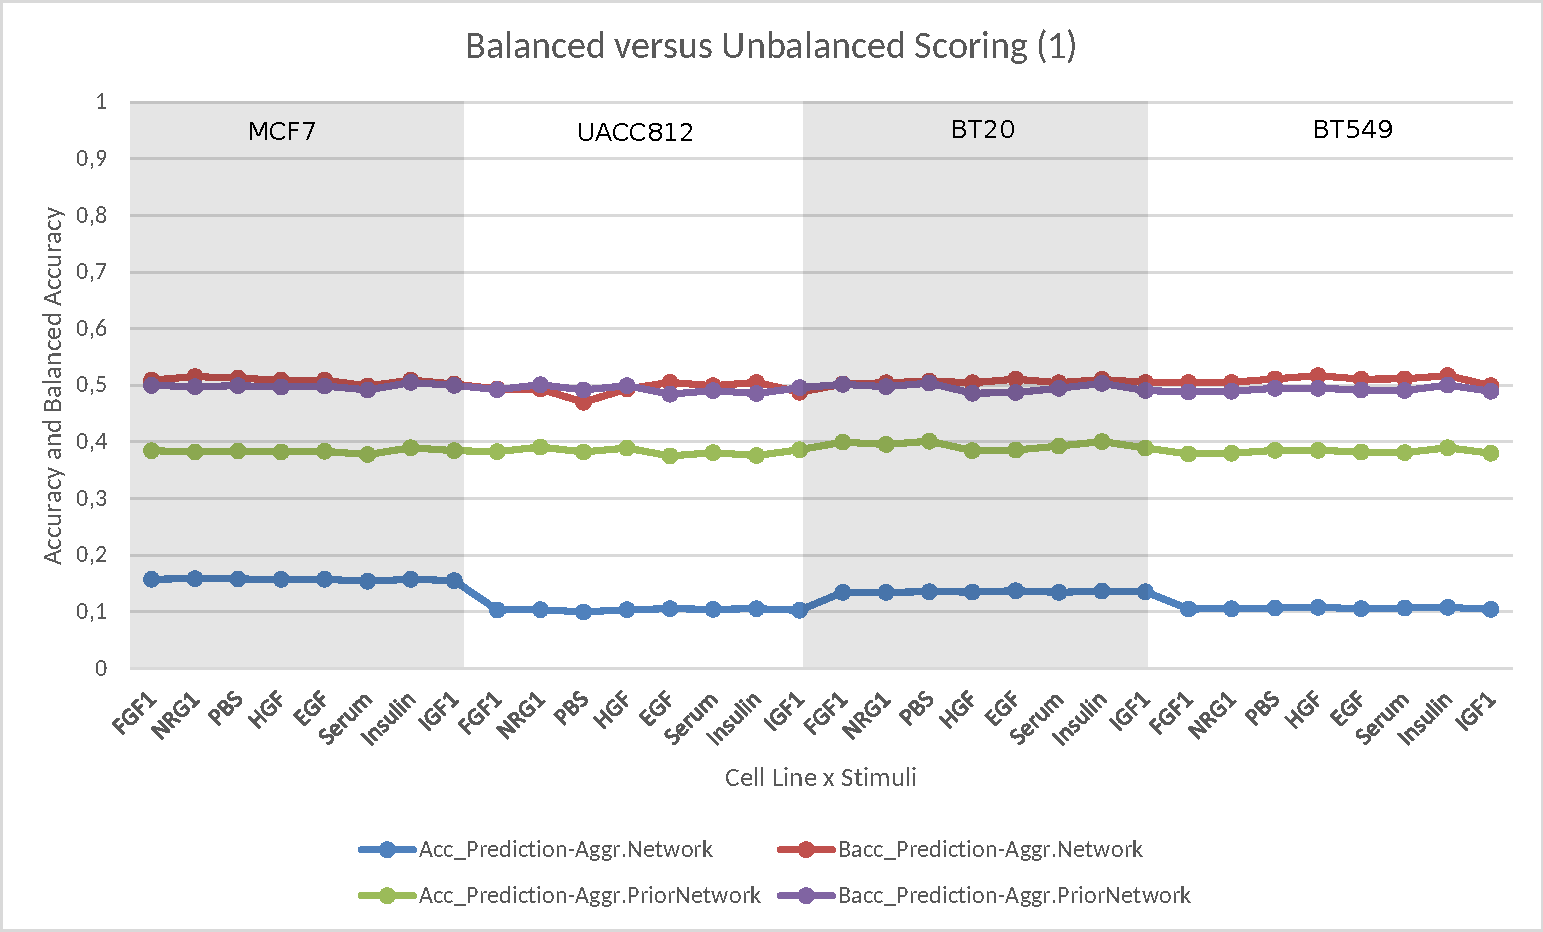
\includegraphics[width=0.9\textwidth]{./Bilder/Scoring/dreamchallenge/1_Balanced_vs_Unbalanced/balanced1.pdf}
\caption[Imbalanced classes (1)]{Imbalanced classes (1). Accuracy and Balanced Accuracy for the prediction scored against the aggregated network and aggregated prior network.}
\label{fig:10}
\end{figure}

This observation is emphasized by considering the size of each class in the confusion matrix for both evaluation measurements. Comparing the prediction with the aggregated network predominantly many false negatives are detected, thus the accuracy is worse. Whereas comparing the prediction with the aggregated prior network the number of false negatives is much lower and the number of true negatives is much higher such that the accuracy yields better result. \\\\

For emphasizing this observation the prediction is scored in Figure 3.10 instead against the aggregated prior network against a submission of the last participant (rank: 74., $\sim 600$ edges among the 32 contexts) of the DREAM8-Challenge leader board \citep{authornamenotavailable}. Here, scoring the prediction against the last participant shows that the disparity of the size between these networks is not that big as between the prediction and the aggregated network. Thus scoring the prediction against the last participant results in a predominant abundance of true negatives thus the mean accuracy of $\sim 0.716$ is much better than scoring the prediction against the aggregated network.

\begin{figure}[H]
\captionsetup{width=0.9\linewidth}
\centering
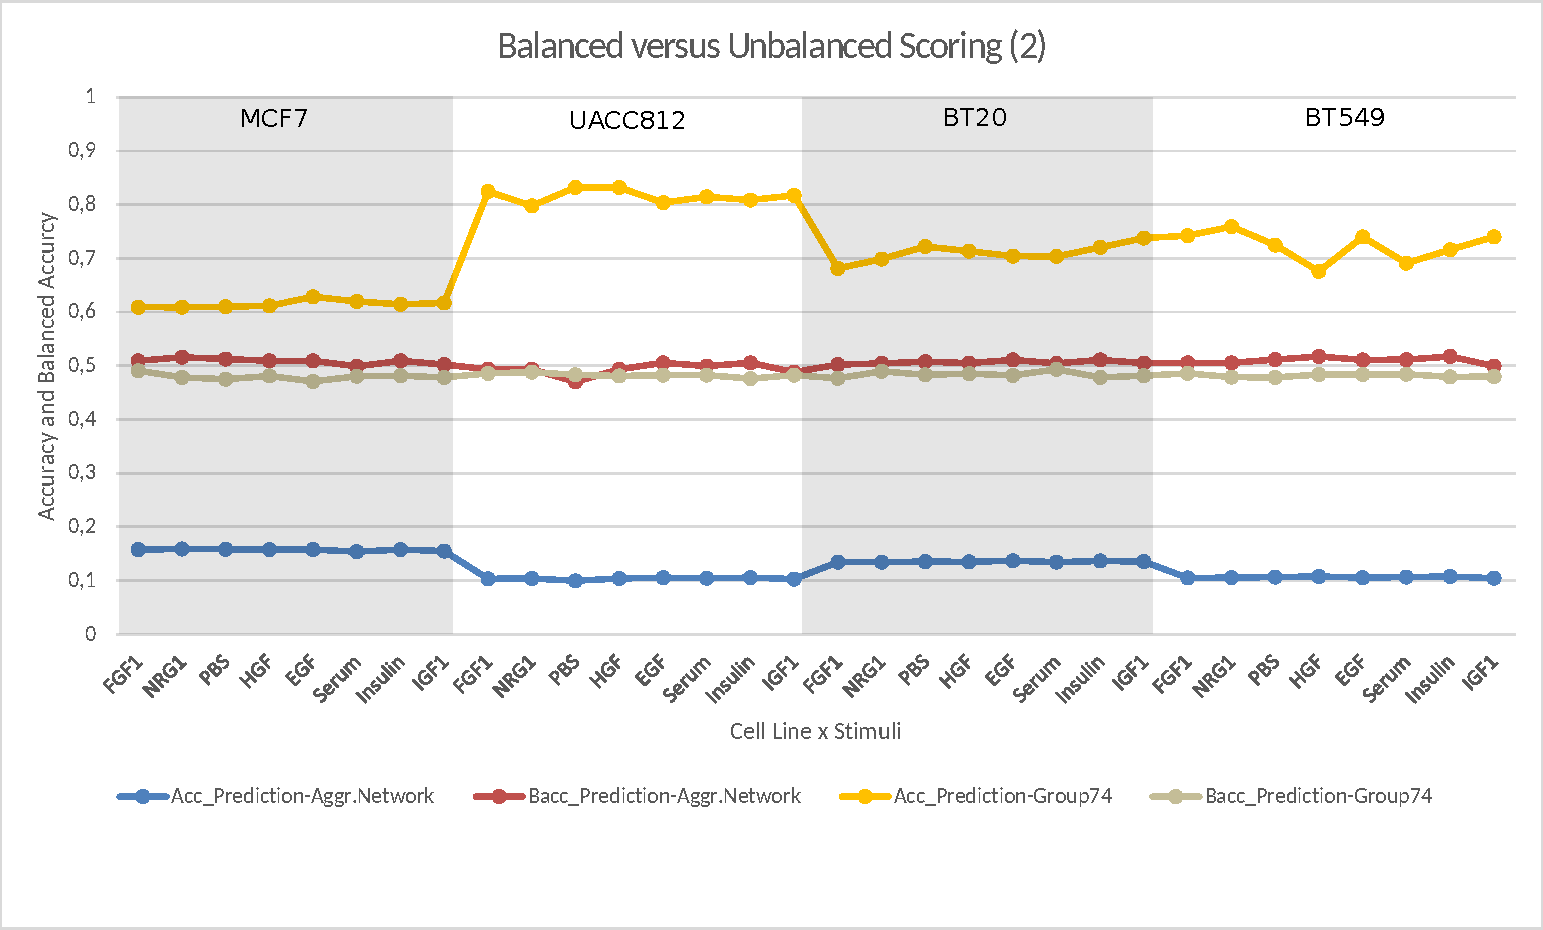
\includegraphics[width=0.9\textwidth]{./Bilder/Scoring/dreamchallenge/1_Balanced_vs_Unbalanced/balanced2.pdf}
\caption[Imbalanced classes (2)]{Imbalanced classes (2). Accuracy and Balanced Accuracy for the prediction scored against the aggregated network and aggregated prior network.}
\label{fig:10}
\end{figure}

The impact of true negatives and false negatives can be put into perspective by applying the balanced accuracy metric. Therefore accuracy is neglected and further evaluation are perfomed with precision, recall, balanced accuracy and matthew correlation coefficient.\\


In Figure 3.11 the recall (a) and the precision (b) values are shown. It is important to indicate that the recall is presented in a higher resolution such that each evaluation is easier to distinguish.\\


\begin{figure}[H]
\captionsetup{width=0.9\linewidth}
\centering
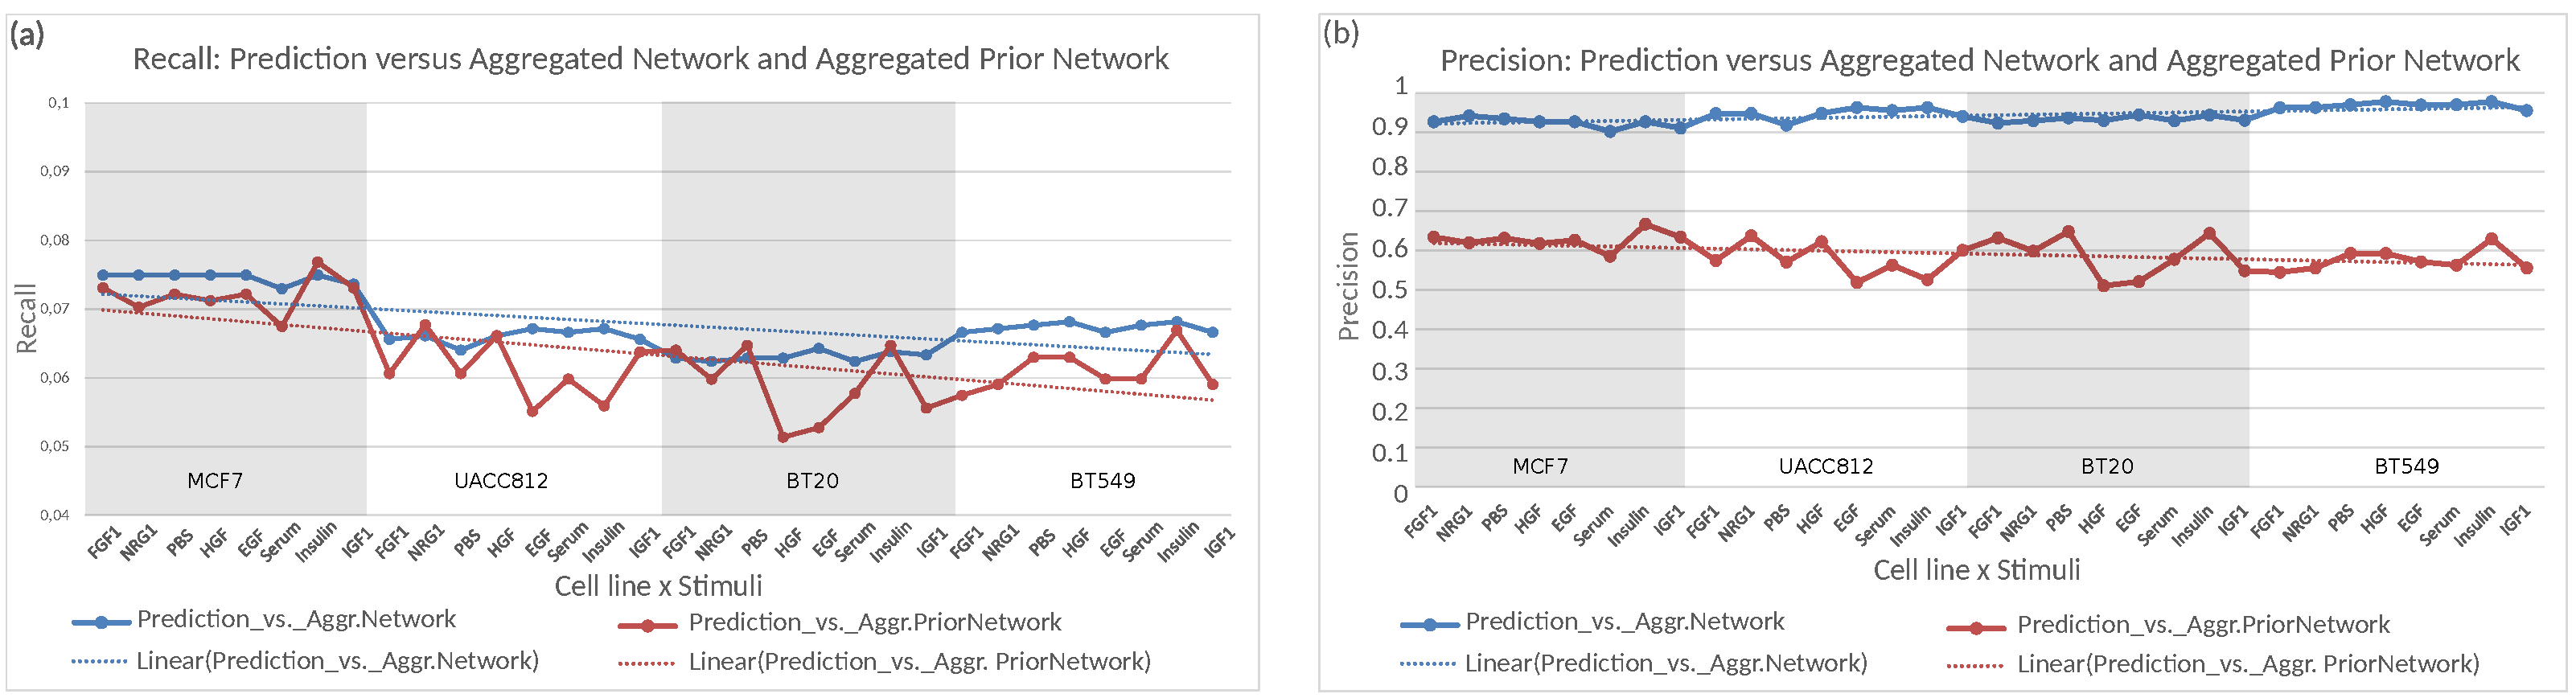
\includegraphics[width=1.0\textwidth]{./Bilder/Scoring/dreamchallenge/1_Balanced_vs_Unbalanced/balanced_recprec.pdf}
\caption[Recall: Prediction versus Aggregated/Prior Network]{Recall: Prediction versus Aggregated/Prior Network}
\label{fig:10}
\end{figure} 

In (a) the prediction is scored against the aggregated network yielding a mean recall value of $\sim 6,7\%$ and scored against the aggregated prior network resulting in a mean recall value of $\sim 6,3\%$. Beside the fact that scoring against the aggregated prior network causes a few fluctuations among cell lines and stimuli the overall mean recall value is not significantly different to the mean recall value of scoring the prediction against the aggregated network. All in all, the prediction predicted $\sim 6,5\%$ of the releveant elements.\\
In (b) the prediction scored against the aggregated network yields a mean precision value of $\sim 0.943$, meaning about $\sim 94,3\%$ edges are predicted correctly. Regarding the prediction beeing scored against the aggregated prior network regarding the mean precision value about $\sim 59,1\%$ edges are predicted correctly. 
%The aggregated network is much bigger than the prediction and much bigger than the aggregated prior network (Table 3.2). Thus, the aggregated network builds a bigger intersecting set of true values covering most of the predicted elements.

\subsection*{New Ranking: Aggregated Network and Aggregated Prior Network}

A total of $74$ submissions of participants of the DREAM8-Challenge in combination with the predicted network of the DREAM8-Challenge pipeline are scored against the aggregated network and the aggregated prior network. The networks are ranked by their mean value of balanced accuracy, Matthew correlation coefficient (Mcc), precision and recall such that a ranking of the prediction is achieved. 

In Figure 3.12-3.14 names of the participating groups of the DREAM8-Challenge are pseudonymized by their original ranking of the SC1A leaderboard.
%\citep{https://www.synapse.org/#!Synapse:syn2289138}. 
%Im Anhang Leaderboard 
For this reason the prediction of the DREAM8-Challenge is pseudonynomized by a value of $0$, which is highlighted in each figure by a red rectangle. In Table 3.3. the ranking of the prediction for each evalutaion method and its corresonding value is shown.


\begin{table}[H]
\begin{center}
%\captionsetup{width=0.87\linewidth}
%\scriptsize
\small
\begin{tabular}{l|c|c|c}
\toprule 
\textbf{Scoring metric} &\textbf{Type} & \textbf{Aggregated Network} & \textbf{Aggregated Prior Network}\\
 \hline\hline
\rowcolor{black!10} Mean Balanced Accuracy & rank & 43 & 49\\
  & value & $\sim 0.0628$ &$\sim 0.4950$\\
\rowcolor{black!10} Mean Mcc & rank & 33 & 39\\
  & value &$ \sim 0.0097$ &$ \sim 0.0195$\\
\rowcolor{black!10} Mean Precision & rank & 33 & 45 \\
 & value & $\sim 0.9436$& $\sim 0.5909$\\
\rowcolor{black!10}Mean Recall & rank & 42 & 47\\
  & value & $\sim 0.0677$ & $\sim 0.0632$\\
\bottomrule
\end{tabular}
\captionof{table}{Ranking of the prediction}
\end{center}
%}
\end{table} 

In Figure 3.12 mean balanced accuracy values are descend ordered by the values of all submissions and the prediction scored against the aggregated prior network. In relation to the DREAM8-Challenge submissions the prediction has a rank of 49 with a value of $\sim 0.495$. Mean balanced accuracy values ordered by the aggregated network yields a rank of 43 for the prediction with a value of $\sim 0.063$.\\%Grund: FN so immens hoch, sodass selbst BACC das nicht mehr relativieren kann.
Regarding the mean Matthew-correlation-coefficient in Figure 3.13 the networks are descend ordered by the results of scoring against the aggregated network. For this case the prediction yields a new rank of 33 with a value of $\sim 0.0097$ and values ordered by scoring against the aggregated prior network yield a rank for the prediction of 39 and a corresponding value of $\sim 0.0195$.


Regarding the mean recall ranking in Figure 3.13 the ranking is ordered by the scoring against the aggregated prior network, and the prediction predicts $\sim 6,8\% $ of relevant edges of the aggregated network with a rank of 42 and predicts $\sim 6,3\% $ of relevant edges of the aggregated prior network with a rank of 47.\\ 
Furthermore, the precison shows that regarding the aggregated network the prediction predicts $\sim 94.36\%$ of the relevant edges correctly with a rank of 33 and regarding the aggregated prior network the prediction predicted $\sim 59,1\% $ of the relevant edges correctly with a rank of 45.\\\\ 

Averaging across the whole evaluation set for scoring against the aggregated network the prediction  yields a rank of 49 and for scoring against the aggregated prior network the prediction yields a rank of 50.
It is noticed that averging among the whole evaluation set captures the ranking of the best performing group in the DREAM8-Challenge. This control emphasizes the reliability of evaluation methods used in this thesis.

% Balanced Accuracy
\begin{figure}[H]
\centering
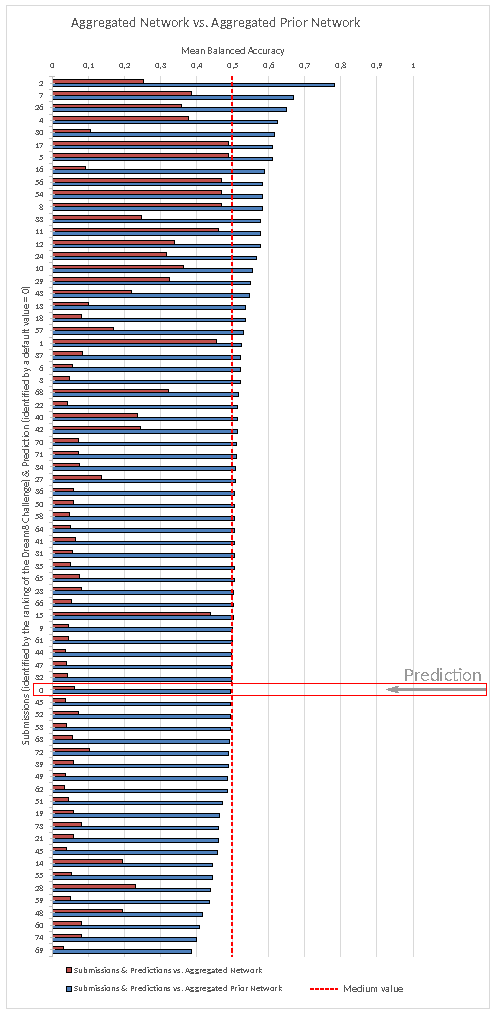
\includegraphics[width=0.7\textwidth]{./Bilder/Scoring/dreamchallenge/Meanbacc_vertical_comparison2.pdf}
\caption[New Ranking Balanced Accuracy]{New Ranking (Balanced Accuracy): Aggr. Network and Aggr.Prior Network}
\label{fig:}
\end{figure}


%MCC
\begin{figure}[H]
\centering
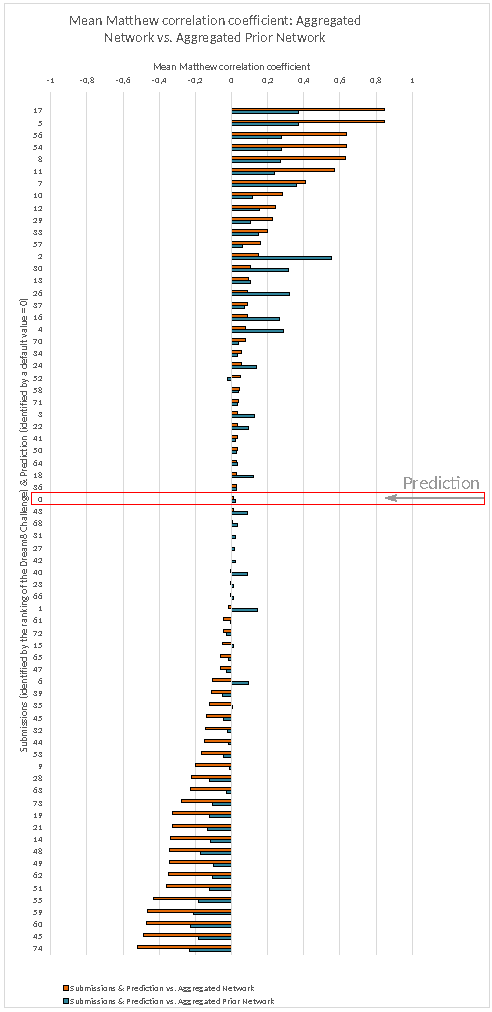
\includegraphics[width=0.7\textwidth]{./Bilder/Scoring/dreamchallenge/MeanMcc_vertical_comparison2.pdf}
\caption[New Ranking: Matthew correlation coefficient]{New Ranking (Matthew correlation coefficient): Aggr. Network and Aggr.Prior Network}
\label{fig:}
\end{figure}

%Precision and Recall
\begin{figure}[H]
\centering

\includegraphics[width=0.82\textwidth]{./Bilder/Scoring/dreamchallenge/Recall_Precision_vertical_comparison.pdf}
\caption[New Ranking: Precision and Recall]{New Ranking (Precision and Recall): Aggr. Network and Aggr.Prior Network}
\label{fig:}
\end{figure}






    \clearpage{\pagestyle{empty}\cleardoublepage}
    \chapter{Results}



\section{}

\begin{figure}[H]
\centering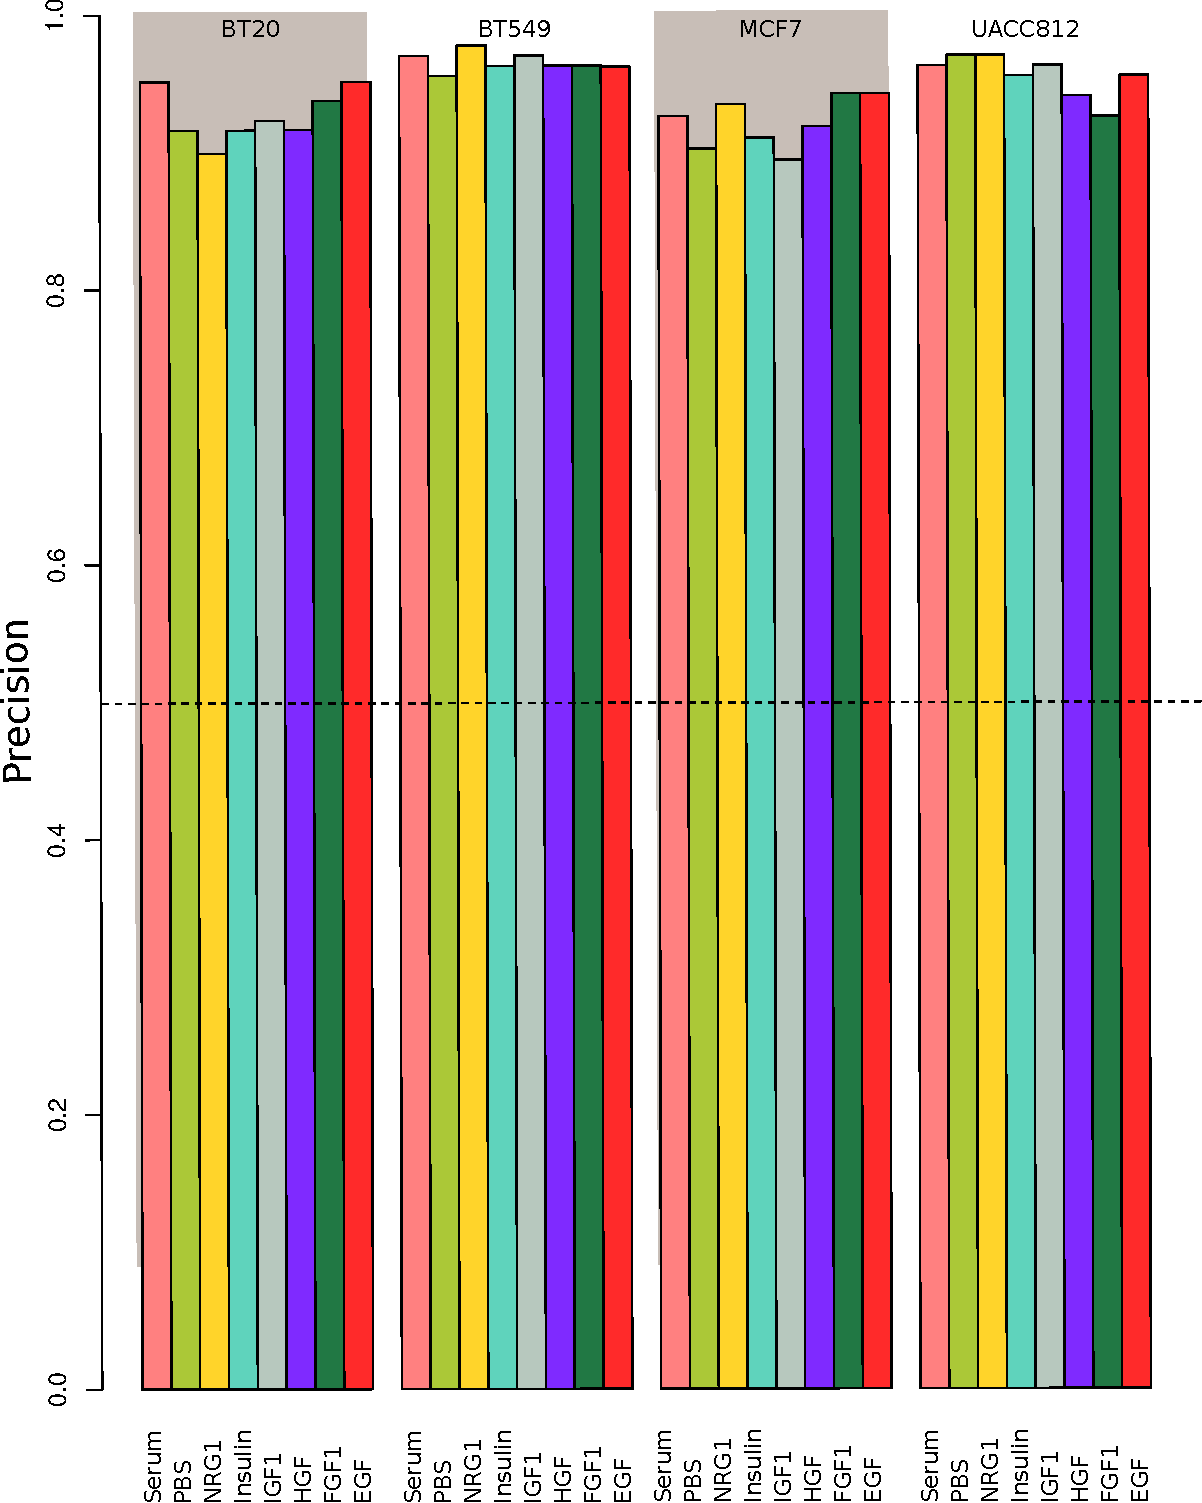
\includegraphics[width=0.4\textwidth]{./Bilder/Precision.pdf}
\caption[Precision]{ }
\label{fig:}
\end{figure}


\section{}


\section{}


    \clearpage{\pagestyle{empty}\cleardoublepage}
    \chapter{Conclusion}
%Preprocessing

%TS2B:%Quelle: TS2B-Paper/ Error-Assessment-Paper

%Nachteile von BooleanModels:
%- Recent survey say: "Faithfulness to biological reality", "ability to model dynamics"is low
%- TS2B needs a relatively large number of time points in the time-series data, otherwise we have the problem of "too many variables, too few equations", which a very large degree of freedom, thus a nonuniqueness of solutions.
%- In practice the regulatory network is unknown, thus judging whether a BN provides a close approximation or notis not easy.
%- ODE's are used to simulate the "true dynamics", but ODE's are not necessarily unique with respect to the dynamics they generate
%- It is important to mention,that often the goldstandard network is constructed from multiple informtion (literature, mature information).In this case just the raw time-series data was provided without additional information.
%- Parameter of the model have a big effect:e.g. Initial concentration in the time-series data set: Has significant influence on the topology and functions of the inferred BN. For instance: if the reaction rate is quite low the dependecy of two genes cant be observed in the synchronous documented time-series.
%-\citep{CHAI201455}: BN-based methods are not suitable for large-scale network inference,because allpossible combinations of genes were exhaustivley compared so as to find a best of regulatory genes for a given target gene. (e.g. Bestfit, REVEAL)

%Vorteil:
%- Very closely reflecting the topology of a regulatory network (upstream/downstream relationships)
%- faithfulness to biological reality: Binarization, redundancy removal -> varying degrees
%- number of Boolean functions is exponential in the number of genes in the system

%General:
%- The more complex a system is (heavily oscillatory,large variability) the more time points are needed.
%- BN have a good predictive power for small networks
% Fast convergence of BESTFIT can be explained by its lack of requirement that the candidate functions f' be complete.
% Slow Convergence: REVEAL only accepts complete functions, thus R. produces more intuitive BN


%Finally:
%- The amount of time-points at which concentrations maust be sampled may be very large (with disagrees with commonly stated claim that BN require very little data to learn or train.)

%Improvements & Outlook:\citep{CHAI201455} 
% - There are several other boolean algorithms for network modeling:
% - Baysian inference approach for a Boolean Network(BIBN): The maximum number of regulatory genes is bounded by two and used to infer a Boolean network by maximizing a joint posterior probability. To select the most informative regulatory genes an approximated multivariate mutual information measure is inccorporated.
%- ARCANE: Time-delay algorithm for the reconstruction of accurate cellular networks (ARCANE) method is used to compute the mutual information by considering a time gap between gene expression values.\citep{Zoppoli2010}
%MIDER: Mutual information distance and entropy reduction method (MIDER),which defines a mutual information-based distance between genes to specify the directionality.\citep{10.1371/journal.pone.0096732}
%- MIBNI: Mutual information-based Boolean network inference method:The method first identifies a et of initial regulatory genes using mutual information-based feature selection, andthen improves the dynamics prediction accurary by iteratively swapping a pair of genes betweensets of the selected regulatory genes and the other genes. (good for structural and dynamic analysis)\citep{10.1371/journal.pone.0171097}
%- Kombination aus Boolean Approach und ODE: First break down the complex system to low level informative network. Attractor analysis. Then focus on the nodes of the attractor and the basinsand then just look by ODE on the smaller subset of nodes.(e.g. kinetic information)

%- GROßER NACHTEIL:
%These mutual information-based methods are computationally expensive, because they are implemented to compute exact mutual information values over all possible combination of genes.

%Quelle: https://www.nature.com/articles/nmeth.3773
%- In insilico data network inference were almost better inferred when teams did not use prior knowledge.
%- Conversely, notusing a prior network did not necessarily result in poor performance; mean AUROC scores ranged from 0.49-0.71, with prior knowledge: 0.49-0.78.
%- Similar previous DREAM challenges showed that there is no clear relationship between method (inference algorithm) and performance. Pre-processing and implementation are important.
%- With the aggregated prior network potentially novel changes can be highlighted.
%- Although causal network inference mayfail for many theoretical and practical reasons, the results of this challenge showed, that it is feasible inferring significant large-scale networks in complex mamalian settings by a community effort.
%- it is emphasized that further work needed to clarify the theoretical properties of the score.
%Result: Their analysis revealed contexts that deviate from known biology, such deviations are likely to be particularly important for understanding disease-specific dysregulation and therapeutic heterogenity. Furthermore, it is possible that the literature is biased toward cancer, and for that reason priors based onthe literature may be less effective in other disease settings.

% DREAM Challenge:Additional Data Details
% Quelle:https://www.synapse.org/#!Wiki:syn1720047/ENTITY/56210
% - Some phopsho antobodies have low quality and should be xcluded from the set
% - Annotation error might cause wrong scoring against the gold standard
% - Antibodies are NOT comparable. Each antibody has varying degrees of affinity and avidity towards its target protein. Assuming two proteins have the same concentration, they may not result in the same level of data values. Therefore, they are not directly comparable.
% - Batch Effect: Samples in different cell lines are NOT comparable (e.g. the datapoint for AKT_pS473 in MCF7 (serum,5min,DMSO) can not be compared with the corresponding datapoint in BT20).Normalization procedures could be used to reduce the batch effect.
% - The antibodies available for this assay have evolved over time, so the proteins measured are not identical across all datasets. (BT20 = 48, BT549 = 45, MCF7 = 41, UACC812 = 45 phophoproteins)
% - Some antibodies target more than one isoform of a protein (eg: the antibody for AKT targets AKT1, AKT2, AKT3)
    \clearpage{\pagestyle{empty}\cleardoublepage}

% -----------------------------------
%\backmatter 
\bibliographystyle{apacite}				% bei natbib in deutsch
\bibliography{./Literatur/quellen}		% Literaturquellen einbinden 
\newpage
\thispagestyle{empty}

\section*{Declaration of Originality}

\vspace*{2cm}

\noindent
I hereby declare that this thesis and this work reported herin was composed by and originated entirely from me. 
\\\\
Information derived from published and unpublished work of others has been acknowledged in the text and references are given in the list of sources.

\vspace{2cm}

\noindent
Berlin, November 20,2018
\vspace{2cm}
%\vspace{3cm}

%\hspace*{7cm}%
%\dotfill\\
%\hspace*{8.5cm}%
Nina Valery Kersten


 			% Eidesstattliche Erkl�rung (nicht bei Seminararb.)

\end{document}
